\documentclass[10pt]{article}

% --- 1. CONFIGURAZIO OROKORRA (UPV/EHU) ---
\usepackage[a4paper, total={170mm,257mm}, top=2.5cm, bottom=2.5cm, left=2.5cm, right=2.5cm, headsep=1cm]{geometry}

\usepackage[dvipsnames]{xcolor}
% Definimos los colores AQUÍ, al principio, para evitar errores
\definecolor{codegray}{rgb}{0.9, 0.9, 0.9}
\definecolor{light-gray}{gray}{0.87} 
\definecolor{shadecolor}{RGB}{240, 240, 240} 

\usepackage{lipsum}
\usepackage{framed}
\usepackage{graphicx}
\usepackage{afterpage}
\usepackage{fontspec} 
\usepackage{textcomp} % Para símbolos especiales

% Solución robusta para la virgulilla (~) en la bibliografía
\newcommand{\texttilde}{\ensuremath{\sim}}

\usepackage{parskip}
\usepackage{indentfirst}
\setlength{\parindent}{1.5em}
\usepackage{ragged2e}
\usepackage[basque]{babel}
\usepackage{microtype}
\usepackage{amsmath}

% Hyperref al final para evitar conflictos
\usepackage[colorlinks=true, linkcolor=blue, citecolor=blue, urlcolor=blue]{hyperref}
\usepackage{tabularx}
\usepackage{array}
\usepackage{acronym} 
\usepackage{listings} 
\usepackage{comment}
\usepackage{float} % Para posicionar mejor las imágenes (H)

\usepackage{tikz}
\usetikzlibrary{trees}

% --- 2. FUENTES (EHUSerif) ---
% Si falla la carga de fuentes, comenta este bloque temporalmente
\setmainfont{EHUSerif-Light.otf}[ 
  Path = ./EHU Serif/,                        
  BoldFont = EHUSerif-Bold.otf,      
  ItalicFont = EHUSerif-Italic.otf, 
  BoldItalicFont = EHUSerif-BoldItalic.otf, 
]
\newfontface\lightfont{EHUSerif-Light.otf}[Path=./EHU Serif/]
\newfontface\blackfont{EHUSerif-Black.otf}[Path=./EHU Serif/]

% --- 3. ESTILOS CÓDIGO ---
\lstdefinestyle{myArduino}{
  language=C++, 
  morekeywords=[1]{},                   
  morekeywords=[2]{FILE_WRITE},         
  morekeywords=[3]{SD, File},           
  morekeywords=[4]{open, exists},       
  frame=shadowbox,
}

\lstdefinestyle{terminal}{
    backgroundcolor=\color{codegray},
    basicstyle=\scriptsize\ttfamily,
    breaklines=true,
    frame=single,
    columns=fullflexible,
    keepspaces=true,
    showstringspaces=false,
    inputencoding=utf8,
    extendedchars=true
}

% --- 4. FORMATO ---
\usepackage{caption}
\DeclareCaptionLabelFormat{numeroPrimero}{#2. #1}
\captionsetup[figure]{labelformat=numeroPrimero}
\captionsetup[table]{labelformat=numeroPrimero}

% --- 5. TITULOS ---
\usepackage{titlesec}   
\titleformat{\section}
  {\normalfont\Large\bfseries\centering} 
  {\thesection.}{1em}{} 
  [\vspace{0.5ex}\titlerule] 
\titlespacing*{\section}{0pt}{2ex}{2ex}
\newcommand{\sectionrule}{\noindent\titlerule\vspace{0.5ex}} 


% ==========================================
%           DOCUMENTO
% ==========================================
\begin{document}

% --- PORTADA ---
\begin{titlepage}
\hspace*{-3.5cm}
    \begin{minipage}{\textwidth}
        \vspace{-2.5cm}
        \begin{center}
            % Comprobación de seguridad para la imagen
            \IfFileExists{Irudiak/LogoEHU.PNG}
            {
\includegraphics[width=\paperwidth]{Irudiak/LogoEHU.PNG}}
            {} 
        \end{center}
    \end{minipage}

\vspace{1cm}

\hspace{-3.1cm}
\noindent\fcolorbox {light-gray}{white}{
    \parbox{\paperwidth}{
     \begin{center}
     \large Gradu Amaierako Lana \\
     \large Ingeniaritza Elektronikoko Gradua
    \end{center}
    }
}

\vspace{0.8cm}

\noindent\hspace*{-2.5cm}%
\colorbox{light-gray}{\begin{minipage}{\paperwidth}%
    \vspace{1cm}
    \color{RoyalBlue}
    \centering\Large\textbf{ \textit{LoRa}n oinarritutako sentsore sare malgu baten eraikuntza} \\
    \vspace{8cm}\mbox{}
  \end{minipage}
}

\begin{flushright}
 Egilea: \\ \textbf{Gontzal Arregi Aranoa} \\ \vspace{0.5cm}
 Zuzendariak: \\ Iñigo Arredondo López de Guereñu \\ Francisco Javier Echanove Arias \\
\end{flushright}

\begin{center}
\noindent\fcolorbox {white}{white}{
    \parbox{11cm}{
         \begin{center}
            \footnotesize © 2026 Gontzal Arregi Aranoa
        \end{center}
    }
}
\end{center}

\hspace{-3.2cm}
\noindent\fcolorbox {light-gray}{white}{
    \begin{minipage}[]{1000pt}
        \parbox{\paperwidth}{
            \begin{center}
                 Leioa, 2026ko otsailaren 12an
            \end{center}
        }
    \end{minipage}
}
\end{titlepage}

\clearpage
\thispagestyle{empty}
\null
\clearpage

\tableofcontents
\newpage

% --- AKRONIMOAK ---
\section*{Akronimoak}
\begin{acronym}
    \acro{IoT}{Internet of Things (Gauzen Interneta)}
    \acro{LoRa}{Long Range}
    \acro{LoRaWAN}{Long Range Wide Area Network}
    \acro{MQTT}{Message Queuing Telemetry Transport}
    \acro{WSL}{Windows Subsystem for Linux}
    \acro{USB}{Universal Serial Bus}
    \acro{GrAL}{Gradu Amaierako Lana}
    \acro{WHO}{World Health Organization}
    \acro{RH}{Relative Humidity}
    \acro{PM}{Particulate Matter}
    \acro{IDE}{Integrated Development Environment}
    \acro{I2C}{Inter-Integrated Circuit}
    \acro{LCD}{Liquid Crystal Display}
    \acro{NTC}{Negative Temperature Coefficient}
    \acro{Li-Po}{Litio-Polimero}
    \acro{CSS}{Chirp Spread Spectrum}
    \acro{M2M}{Machine to Machine}
    \acro{SDA}{Serial Data Line}
    \acro{SCL}{Serial Clock Line}
    \acro{RSSI}{Received Signal Strength Indicator}
    \acro{SNR}{Signal-to-Noise Ratio}
\end{acronym}
\newpage

\sectionrule
\section{Sarrera}

\subsection{Arazoa}
Materia daukan gauza orok ingurunearekin kontaktua dauka etengabe. Horregatik, gizakiontzako funtsezkoa da inguruneko kondizioari buruzko informazioa edukitzea. Inguruneari buruz gehiago sakonduz, ingurunea bera osatzen duten elementuen artean airea da une oro elkarreragiten ari garen elementua. Ondorioz, airearen kutsadura gure osasunari kalte egiten dion faktore nagusietako bat da. Pertsona gehienek beren eguneroko bizitzaren zatirik handiena espazio itxietan igarotzen dute, bai lanean edo etxean \cite{Klepeis2001}. Horregatik, airearen kalitatea jende askoren kezka nagusienetako bat da, biztanleen osasunean eta ongizatean eragiten baitu. Kutsatzaileen presentziak eta aireztapen desegokiak arazo esanguratsuak suposa ditzakete, osasun arazoak eta bizi baldintzen beheranzkoa eraginez. Izan ere, \textit{\ac{WHO}}ren arabera \cite{qiu2022lung}, airearen kutsadurak zuzenean 3,2 milioi heriotza eragin zituen 2020an, horien artean 200.000 baino gehiago 5 urtetik beherako haurrak izanik.\\

Aire kalitate txarraren ondorioetan sakonduz, aspalditik dakigu hezetasuna dela lizuna sortzeko arrazoi nagusia. Espazio itxietan, hala nola komunak, sukaldeak edo isolamendu gutxiko hormak, hezetasunak baldintza egokiak eskaintzen dizkie onddoei eta lizunei. Giro epel eta hezean, mikroorganismo hauek azkar ugaldu daitezke eta horrek osasun-arazo ugari sor ditzake. Lizunak eragin ditzake alergiak, eztula, sinuen hanturak, begi eta azaleko narritadurak, baita arnasketa gaixotasunak ere. Bereziki kaltegarriak izan daitezke haur txikientzat, adinekoentzat eta arnas gaixotasunak dituzten pertsonentzat \cite{WHO2009}. \\

1953an esperimentu bat egin zen hainbat materialetan lizuna sortzeko inpaktua aztertzeko \cite{block1953humidity}. Airearen egoera aspalditik dagoen kezka bada ere, gaur egun ere, fenomeno horri aurre egiten jarraitzen da. Adibidez, duela gutxi, \textit {Florida 's Premier Energy Research Center}k lizunaren hazkundearen arrazoiak aipatzen zituen artikulu bat argitaratu zuen \cite{ross2021sunbelt}. Adibidez, artikuluan agertzen den gomendioetako bat ondokoa da: udako hilabete beroetan, aire girotua piztuta dagoela, \ac{RH}ak ezin du \%55a gainditu egunean zehar, aipatutako muga oso altua izan barik. Hala ere, klima epela denean, kanpoko hezetasuna ia \%100 \ac{RH}ra irits daitekeela ere nabaritzen dute, eta, kasu horietan, zure etxea kanpora irekita badago, bertako materialek oso heze dagoen aire horren hezetasuna xurgatuko dute. Gainera, hezetasun hori hurrengo egunean ezabatzen ez bada, zure etxeko materialen ''uraren jarduera'' \%75ean edo hortik gora manten daiteke denboraldi luzeetan, eta litekeena da lizuna haztea gainazal horietan. Horregatik, hezetasuna eta tenperatura kontrolatzen dituen sentsore motaren bat instalatzea gomendatzen dute artikulu honetan bertan.\\

Gaur egun, gure inguruneari buruzko informazioa ematen duten soluzioak kasu gehienetan bakanduta daude, eta, monitorizazio sistema aproposak lortzeko, aditu baten esku-hartzea ezinbestekoa izan ohi da. Horrenbestez, erabiltzaile arruntek hezetasuna eta tenperatura kontrolatzeko zailtasun handiak izan ohi dituzte.\\

Horrenbestez, aipatutako premiazko erronka horiei erantzuteko, \ac{GrAL} honen helburua gure inguruneko datuak jasoko dituen sentsore sare malgu bat diseinatzea izango da.\\

Beraz, sistema honen bidez gure ingurunearen kondizioa monitorizatzeko modua bilatuko da, soluzio integratu bat eskainiz. Horretarako, erraz eskuratu daitezkeen gailuak eta askea den software-a erabiliko dira.\\

\subsection{Inguruneko datu-prozesaketari dagokionez gaur arteko kanpo-lana }
\label{sec:Aire kalitateari dagokionez gaur arteko kanpo-lana }

\ac{LoRa} sare malgua diseinatu aurretik, gaur arte dauden baliabideei buruzko ikerketa bat egin da, \ac{GrAL}a inplementatzeko beharra berresteko. Adibidez, \textit{Letters in Applied Microbiology} liburuan \cite{society1992letters}, eskualde hezeetan barne-ingurune higieniko, iraunkor eta lizunik gabea lortzeko egungo erronkak adierazten dituen arazo bat azaltzen da. Artikulu honetan, besteak beste, hezetasun erlatiboaren kontrola \ac{RH}, tenperatura eta mantenugaiak lizuna sortzeko parametro garrantzitsuenak direla azaltzen da. Baieztatzen da, alde batetik, \ac{RH} $>$\%90 izateak lizuna barnealdeetan haztea eragiten duela, eta, beste alde batetik, gizakientzat erosoa den tartearen (19ºC - 24ºC) barnean dauden tenperatura-aldaketek lizunaren hazkundea pixka bat atzeratzea eragiten duela. Gainera, aipatu behar da hainbat erakundek \ac{RH} maila desberdinak gomendatzen dituztela lizunaren hazkundea prebenitzeko. Adibidez, sarreran aipatu bezala, \textit {Florida 's Premier Energy Research Center} ikerketak epe luze batean \%75eko \ac{RH} batek lizuna haztea eragin dezakeela iradokitzen du. Gainera,\textit {\ac{WHO}} \cite{heseltine2009guidelines} ados dago baieztapen horrekin, eta baieztatzen du \ac{RH}ren \%75 har daitekeela muga gisa eraikuntzarako materialetan lizuna haztea eragozteko. Bestalde, Estatu Batuetako \textit{Environmental Protection Agency} \cite{belkin2001haunted} delakoak \%30etik \%60ra bitarteko tartea proposatzen du.\\

Espazio itxietako ingurunearen azterketan murgilduz, 2015ean esperimentu bat egin zen Trenton \cite{marchetti2015campus}, proposatuko dugun antzeko sistema batekin. Kostu txikiko sistema teknologikoak erabili zituzten ikasgeletako airearen kalitatea ebaluatzeko, haririk gabeko sentsore-sareen (WSN) arkitektura bat inplementatuz. Kasu honetan, $CO_2$ kantitatea bakarrik erabili zuten adierazle gisa, kontuan hartu gabe airearen toxikotasuna beste substantzia batzuek eragin dezaketela, hala nola $NO_x$k (oxido nitrikoa eta nitrogeno dioxidoa) edo $NH_3$k (amoniakoa). Beraz, $CO_2$ maila monitorizatzeaz gain, beste substantzia batzuk kontrolatzea komeni da airearen kalitatea behar bezala ebaluatzeko. Hala ere, emaitzek erakutsi bezala, erabilgarria izan daiteke airearen kalitatea barnealdean monitorizatzeko sistema bat erabiltzea. 2019an \cite{son2019correlation}, antzeko beste sistema bat erabili zen estazioen artean airearen kalitatean izandako aldaketak monitorizatzeko. Lan honetan, Arduino mikrokontrolagailuak erabili ziren datuak biltzeko, MQ-135 sentsorea airearen kalitate orokorrerako eta DHT-11 sentsorea tenperatura eta hezetasunerako integratuz. Airearen kalitatea aldagai askoren mende dagoela frogatu zuen, eta, esan bezala, datuak eguneratuta edukitzea ideia ona da erabakiak informazio gaurkotuarekin hartzeko.\\

\ac{IoT}k parte hartzen duen beste kasu bat Barodako (India) Maharaja Sayajirao Unibertsitateak 2022an \cite{kantilal2022iot} egin zuen. ''IoTn Oinarritutako Airearen Kalitatea Monitorizatzeko Sistema, Energiaren Kontsumoa Optimizatuta eta Airearen Kalitatearen Parametroak Ikaskuntza Sakonaren Bidez Iragarrita'' izeneko proiektu honek \ac{IoT} teknologia integratzen du. Hardwareari dagokionez, sistema honek ESP32 mikrokontrolagailua —Wi-Fi eta Bluetooth integratua duena— eta MQ serieko gas-sentsoreak (MQ-131 ozonorako eta MQ-7 karbono monoxidorako) erabili zituen. Protokolo arina da eta gailu bateragarriak erabiltzeak airearen kalitate-parametroak urruneko zerbitzari batera arazorik gabe transmititzea ziurtatzen du. Era berean, proiektuak energia aurrezteko estrategia bat ezartzen du detekzioan eta transmisioa optimizatzen du, datuen iragarpenerako ikasketa sakoneko (\textit{Deep Learning}) ereduak aplikatuz.\\

Lizunaren prebentzioa eta airearen kalitatearen kontrola egiteko, Alaa Alaidroos eta Ibrahim Mosly \cite{alaidroos2023preventing} irakasleek klima bero eta hezeetan aireztapen mekaniko altuak zituzten hezkuntza-eraikinetan ikerketa interesgarria egin zuten. Kasu honetan, sentsore fisikoen ordez, eraikinen simulazio-eredu numerikoak eta VTT lizun-hazkunde eredu matematikoa erabili zituzten aireztapen mekanikoko sistemen (HVAC) errendimendua optimizatzeko. Gurearen antzeko sistemarekin, airearen kalitatea monitorizatzea lortu zuten hainbat okupazio zituzten ikasgeletan, eta, okupazio-maila bakoitzerako aireztapen-tasa optimoak iradokitzeko eredu bat sortu zuten. Klima bero eta hezeetan kokatutako eraikinek, aireztapen mekanikoko tasa handiekin jardunez gero, karga latente handiak jasan zitzaketela ondorioztatu zuten. Eraikinen barnealdera aire fresko eta hezea sartzean, barrualdeko hezetasun-maila altua eragiten du, zeinak lizuna haztea eragiten duen, eta ondorio gisa, osasunerako arriskuak. Beraz, ikerketan lortutako datuak aztertzean, aireztapen optimoaren eta hozte-tenperaturen gutxi gorabeherako balioa lortzen da, zeina oso puntu interesgarria den.\\

Azkenik, airearen kalitate txarra gaixotasun askoren kausa izan daitekeela frogatzen duten ikerketak lortu dira. Adibidez, 2020an, Savannah Michelle Mack, Nicholas Kenyon eta Chao Chenek ikerketa bat egin zuten Kalifornian, Estatu Batuetan \cite{mack2020air}. Ikerketa Imperial Konderriko (Kalifornia) haurren asma tasa altuan zentratu zen, \ac{PM} eta arnasketa-arazoen arteko korrelazioa ikertzeko helburuarekin. Eskualdeak hainbat kutsadura-iturriri aurre egin behar dio, hala nola, nekazaritzarena, mugan dauden ibilgailuen gas isurketena, Mexicali deitzen den hirigunearena eta Salton itsasoko sekzio batena. Partikula finen neurketak egiteko, laser bidezko partikula-kontagailu optikoak (Dylos DC1700) erabili ziren, denbora errealean bereizmen espazial eta tenporal handiko datuak lortzeko. Urte osoan bildutako \ac{PM} laginak aztertuta, ikerketaren helburua, partikula horien konposizioa aztertu eta biztanleen osasunean duten eragin kaltegarriak ulertzea izan zen. Aurkikuntzek \ac{PM}arekiko esposizioak, bereziki alergeno arruntekin batera, erantzun asmatikoak areagotzen zituela iradoki zuten.\\

\subsection{\ac{GrAL}aren proposamena}

Gradu-amaierako proiektu honetan inguruneko aire kalitatea analizatzeko sentsore-sare malgu bat garatu da \ac{LoRa} teknologia erabiliz. Teknologia honek irismen handiko haririk gabeko konexioa eta energia-kontsumo oso txikia eskaintzen ditu. Hori dela eta, oso egokia da urruneko monitorizazio-aplikazio jasangarrietarako.\\

Diseinatutako sentsore-sareak bi modulu nagusi ditu: datuak biltzen dituen modulu zentral bat eta sentsore-modulu bat. Bi moduluak mezuak bidaltzeko eta jasotzeko konfiguratuta daude, eta, horri esker, sarea erraz eta eraginkortasunez heda daiteke.\\

Azkenik, sentsore-sareak bildutako datuak ez dira tokian bakarrik biltegiratzen, hodeian ere prozesatzen dira \ac{IoT} bidez.  Hemendik aurrerako aplikazio guztiak burutzeko \ac{WSL} ingurunean Docker \cite{nickoloff2019docker} izeneko software-an burutuko dira, zeina  modularitatean oinarritutako plataforma den, eta, ondorioz aplikazioen mantentze eta hedapen erraza bermatzen dituen. \\

Azkenengo ataleko lehen pausua nodo zentrala ordenagailu batera konektatzea izango da.
Behin konektatuta dagoela, pythoneko \ac{IDE}a erabiliz \ac{MQTT} komunikazio protokoloa \cite{soni2017survey} inplementatuko da. \ac{MQTT} protokoloa erabiltzearen arrazoiak erreferentzian ondo aipatzen diren arren, laburbilduz, ondokoak dira: Fidagarria, arina eta plataforma askoren bidez implementagarria da.\\
\ac{MQTT} erabiltzeaz gain, Telegraf \cite{chan2019resource} izeneko agentea erabiliz, lortutako datuak Influx DB \cite{naqvi2017time} motatako datubase batera bidaliko ditugu. Modu honetan, erabiltzaileak edozein tokitik interneten bitartez lortutako datuak eskuratzeko aukera izango du.\\

\ac{GrAL} honek erakusten du kontsumo baxuko haririk gabeko teknologia eta \ac{IoT} hodeiko prozesamendua konbinatuz gero, irtenbide iraunkorrak eta eraginkorrak lor daitezkeela ingurumen-monitorizazioan eta antzeko beste aplikazio batzuetan.\\

\noindent Proiektu honen kode iturburu osoa —firmware-a, Python pasarela eta dokumentazioa— GitHub-eko biltegi publiko honetan dago eskuragarri: \url{https://github.com/gontzalarregiaranoa-claude/GrAL_IE_Gontzal}.\\

\newpage

\section{Helburuak eta Faseak}

Proiektu hasieran, hainbat helburu definitu dira. Helburu hauek bete ahal izateko proiektua bost fase nagusitan banatu da, ondoren proiektuaren planifikazioa betetzeko erabiliko direnak.\\

% ---------------------------------------------------------------
% Section 1 - Ikerketaren helburuak 
% ---------------------------------------------------------------
\subsection{GrALaren helburuak}

\ac{GrAL} honetan inguruneko datuak jasoko dituen sentsore-sare bat inplementatuko da, \ac{LoRa} bidez komunikatuko dena. Sentsoreak stand-alone izango dira. Inplementatutako sarea malgua izango da, sarea osatzen duten elementuen kopuruaren kudeaketa dinamikoa izango baita. Azkenik, jasotako datuak erraz ikus daitezke web bidez, Dockerri buruzko InfluxDB + Telegrag + \ac{MQTT} konbinazioa erabiliz.\\

Beraz, helburu nagusia laburbilduz:\\

\begin{shaded}
    \noindent \centering \textbf{\ac{LoRa}n oinarritutako sentsore sare malgu baten eraikitzea; eta, jasotako datuak internet bitartez erraz erakustea.}
\end{shaded}

\vspace{0.25cm}

% ---------------------------------------------------------------
% Section 2 - Faseak 
% ---------------------------------------------------------------
\subsection{Proiektuaren faseak}
\label{sec:faseak}

Aipatutako erronka guztiak burutu ahal izateko bost fase edo zeregin nagusitan banatu da proiektua. Hemen fase bakoitzaren deskribapena bere azpi faseekin batera.\\

\begin{enumerate}

\item{\textbf{Mikrokontrolagailuekin ohitu eta sentsoreen datuak eskuratu.} Definitutako helburu guztiak bete ahal izateko, lehenik eta behin, azpiegitura guztia ulertu beharra dago. Unibertsitateko lau urteetan zehar ez dugu arduinorekin lan egin. Ondorioz, kode irekiko plataforma hau ulertzeko bere errotik hasi beharra dago. Gainera sentsoreen balioak jaso, ulertu eta prozesatu beharko dira.
}
  \begin{enumerate}
    \item{Arduinok bere \ac{IDE}a dauka, \textit{C} eta \textit{C++} programazio lengoaiak erabili ditzakeelarik. Behin programatuta, txartelak guztiz autonomoak izan daitezke. Kasu honetan, \textit{C} eta \textit{C++} programazio lengoaiak ezezagunak dira niretzako, beraz, aipatutako dena ulertu beharra dago.
      
    }
    \item{\textbf{Sentsoreen datuak eskuratu} Sentsore bakoitza mundu bat den heinean, lehenengo, sentsoreak arduino plakara konektatu konexio egokiak eginez. Ondoren, sentsoreen datuak ulertu eta prozesatu.}          
        
  \end{enumerate}

\vspace{0.3cm}
    
\item{\textbf{Arduino plakak \ac{LoRa}ren bidez komunikatzea} Gure sarea bi plakaz osatuta egongo da, eta modulu zentrala eta sentsore modulua prestatu behar dira bi plaken arteko komunikazioa burutzeko}
  \begin{enumerate}
    \item{\textbf{Modulu zentrala.} Hau da hasiera batean ordenagailura \ac{USB}-ren bidez konektatuta egongo den plaka. Haririk gabeko konexioaren bidez, kasu honetan \ac{LoRa} erabiliz, sentsoreen moduluko seinaleak jaso beharko ditu.}
    \item{\textbf{Sentsoreen modulua.} Ordenagailuarengandik independentea izango den plaka. Sentsoreen datuak prozesatu, interpretatu eta bidali beharko ditu.}
 
  \end{enumerate}

\vspace{0.3cm}

\item{\textbf{Software container baten bidez \textit{Komunikazio Protokolo Banandua} + \textit{Agentea} + \textit{Datu Basea}n oinarritutako datuak biltzeko eta monitorizatzeko zerbitzu bat inplementatzea.} Jasotako datuak erraz ikusi ahal izango dira web bidez, aurretik aipatutako konbinazioa erabiliz.
 }
  \begin{enumerate}      
    \item{\textbf{Docker} izeneko Software Containerra \textbf{instalatu ordenagailuan}. Kasu honetan \textit{Windows} sistema eragilea erabili denez, \ac{WSL} erabili beharra dago. Izan ere, Dockerrak errazago funtzionatzen du Linux inguruneetan.}
    \item{\textbf{\ac{MQTT}} (Komunikazio Protokolo Banandua) \textbf{brokerra zabaldu}. Horretarako, EMQX izeneko bitartekaria erabiliko da \cite{bender2021open}. Brokerra hedatzeko pausuak ondokoak izango dira: Nahi diren datuak \ac{MQTT} bidez bidali. Horretarako, Python-en \ac{IDE}a erabiliko da. Horren ostean, modulo zentrala integratu, datuak \ac{MQTT} bidez bidal ditzan. Formatua DBn erabiliko dugunaren modukoa izan behar da.}
    \item{\textbf{InfluxDB} Datu Basea \textbf{Telegraf} izeneko Agentearekin \textbf{zabaltzea}. Bietako edozein zabaltzeko, Docker compose erabiliko dugu. Lehenik influxDB zabalduko da, eta, gero, telegrafak zabalduko dira. Azkenik, sortutako datu-basearekin konektatuko da.} 
  \end{enumerate}

\vspace{0.3cm}

\item{\textbf{Sarearen portaera-testak burutu.} Egindako guztiaren froga esperimentala burutuko da. Seinalearen egonkorasuna bermatzeko eta bi plaken arteko distantzia handia izan ahal dela frogatzeko, beharrezko probak egin beharko dira horrenbestez. Gainera, azkenengo hodeian biltzegiratzeko pausuak inolako arazorik gabe funtzionatu beharko du sentsoreen modulua independentea izanik (beti ere energia-iturri batekin).}    \\    

 
\end{enumerate}

\newpage

\section{Sarea eraikitzen}
\label{chp:arduinoplakakLoRabidezkomunikatzea}

Aurreko atalean \ref{sec:faseak}, sistema osoaren analisi
prozesua azaldu den bezala, kapitulu honetan sistema osoa garatzeko erabili
diren atal guztiak azalduko dira banan banan era sakon eta teknikoago batean. 
Sarea zelan eraiki den azaltzeko, lehenengo, arduinorekin ohitu eta sentsoreen datuak eskuratu behar dira.\\

% ---------------------------------------------------------------
% Section 1 - Arduino
% ---------------------------------------------------------------
\subsection{Arduino}
\label{sec:arduino }

\ac{GrAL}ak era egokian aurrera egiteko, ezinbestekoa da eskuen artean daukagun azpiegitura osoa behar bezala ulertzea. Bestela, hasiera batean ondo ulertu barik funtzio sinpleak egiteko gai garen arren (arduinoren \ac{IDE}a nahiko ulergarria da), exekuzio programa konplexuagoa bihurtzen den heinean, izugarrizko garrantzia hartzen du eskuartean daukaguna ulertzeak.\\

\subsubsection{Definizioa}

Gidaliburuek \cite{herrador2009guia} ondo esaten duten moduan, arduino kode irekiko plataforma elektroniko bat da, software eta hardware erabilerrazean oinarritua. Aipatutakoa posible izateko, proiektua mikrokontrolagailu plaken familia baten diseinuan oinarritzen da.
Gainera, arduinok bere \ac{IDE}a dauka, \textit{C} eta \textit{C++} programazio lengoaiak erabili ditzakeelarik. Behin programatuta txartelak guztiz autonomoak izan daitezke. Kasu honetan, \textit{C} eta \textit{C++} programazio lengoaiak ezezagunak dira niretzako, beraz, bere funtzionamendua ere ulertu beharra dago.\\

\subsubsection{Erabilitako Materiala eta Muntaia}

Proiektu hau burutzeko orduan erabiliko dugun materiala malgua da zentzu batean. Izan ere, erabiliko den ereduan bi sentsore erabiltzen diren arren, sentsore kopurua malgua izango da.
Erabilitako materialaren ikuspegi orokor bat izateko, eta, aplikatuko dugun muntaia era errazago batean ikusteko, ondoko irudia daukagu:\\

\begin{figure}[!htbp]
    \centering
    % Control de errores para la imagen
    \IfFileExists{Irudiak/MUNTAIA GrAL.png}
    {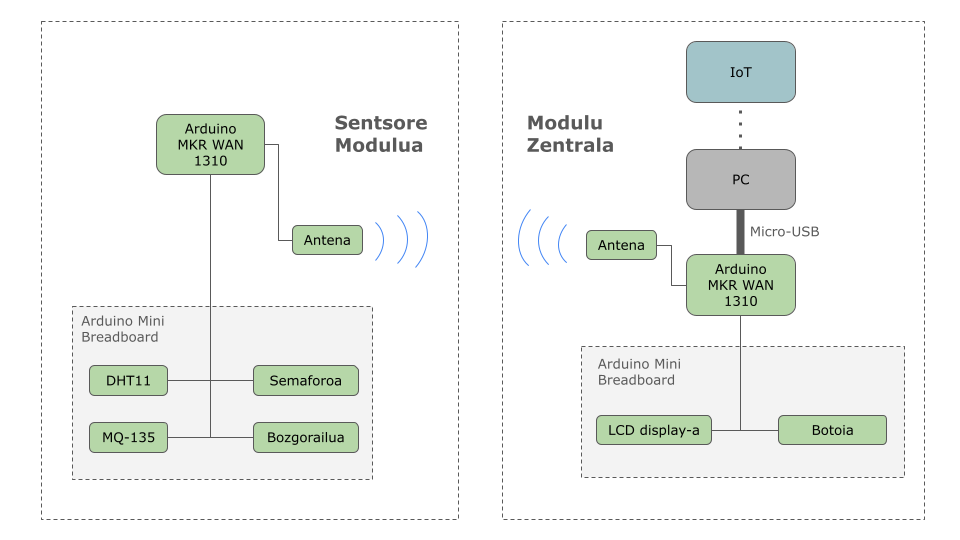
\includegraphics[width=\textwidth]{Irudiak/MUNTAIA GrAL.png}}
    {\fbox{Irudia falta da: MUNTAIA GrAL.png}}
    \caption{Muntaia}
    \label{fig:muntaia}
\end{figure}

Gauzak horrela, erabilitako materialak ondokoak dira:\\

\begin{itemize}

        \item 2X Arduino MKR WAN 1310 
        \label{arduinomkr}
        \item DHT11 sentsorea  %(\hyperlink{DHT}{DHT11 Datasheet})
        \item MQ-135 sentsorea  
        \item Bateria kargagarria
        \item 2X Mini breadboard arduino 400 pin
        \item 2X Antena
        \item \ac{I2C} \ac{LCD}
        \item Bozgorailua
        \item Semaforoa
        \item Erresistentziak  %orain ez dakit zenbat ohm
        \item Kableak
        
\end{itemize}

% --- IMÁGENES REALES DE LOS MÓDULOS ---
\vspace{0.5cm}
Hemen behean ikus daitezke garatutako sistemaren bi modulu nagusien argazki errealak, osagai guztiak konektatuta eta funtzionamenduan daudela:\\

\begin{figure}[H]
    \centering
    \IfFileExists{Irudiak/sentsore_modulua.jpg}
    {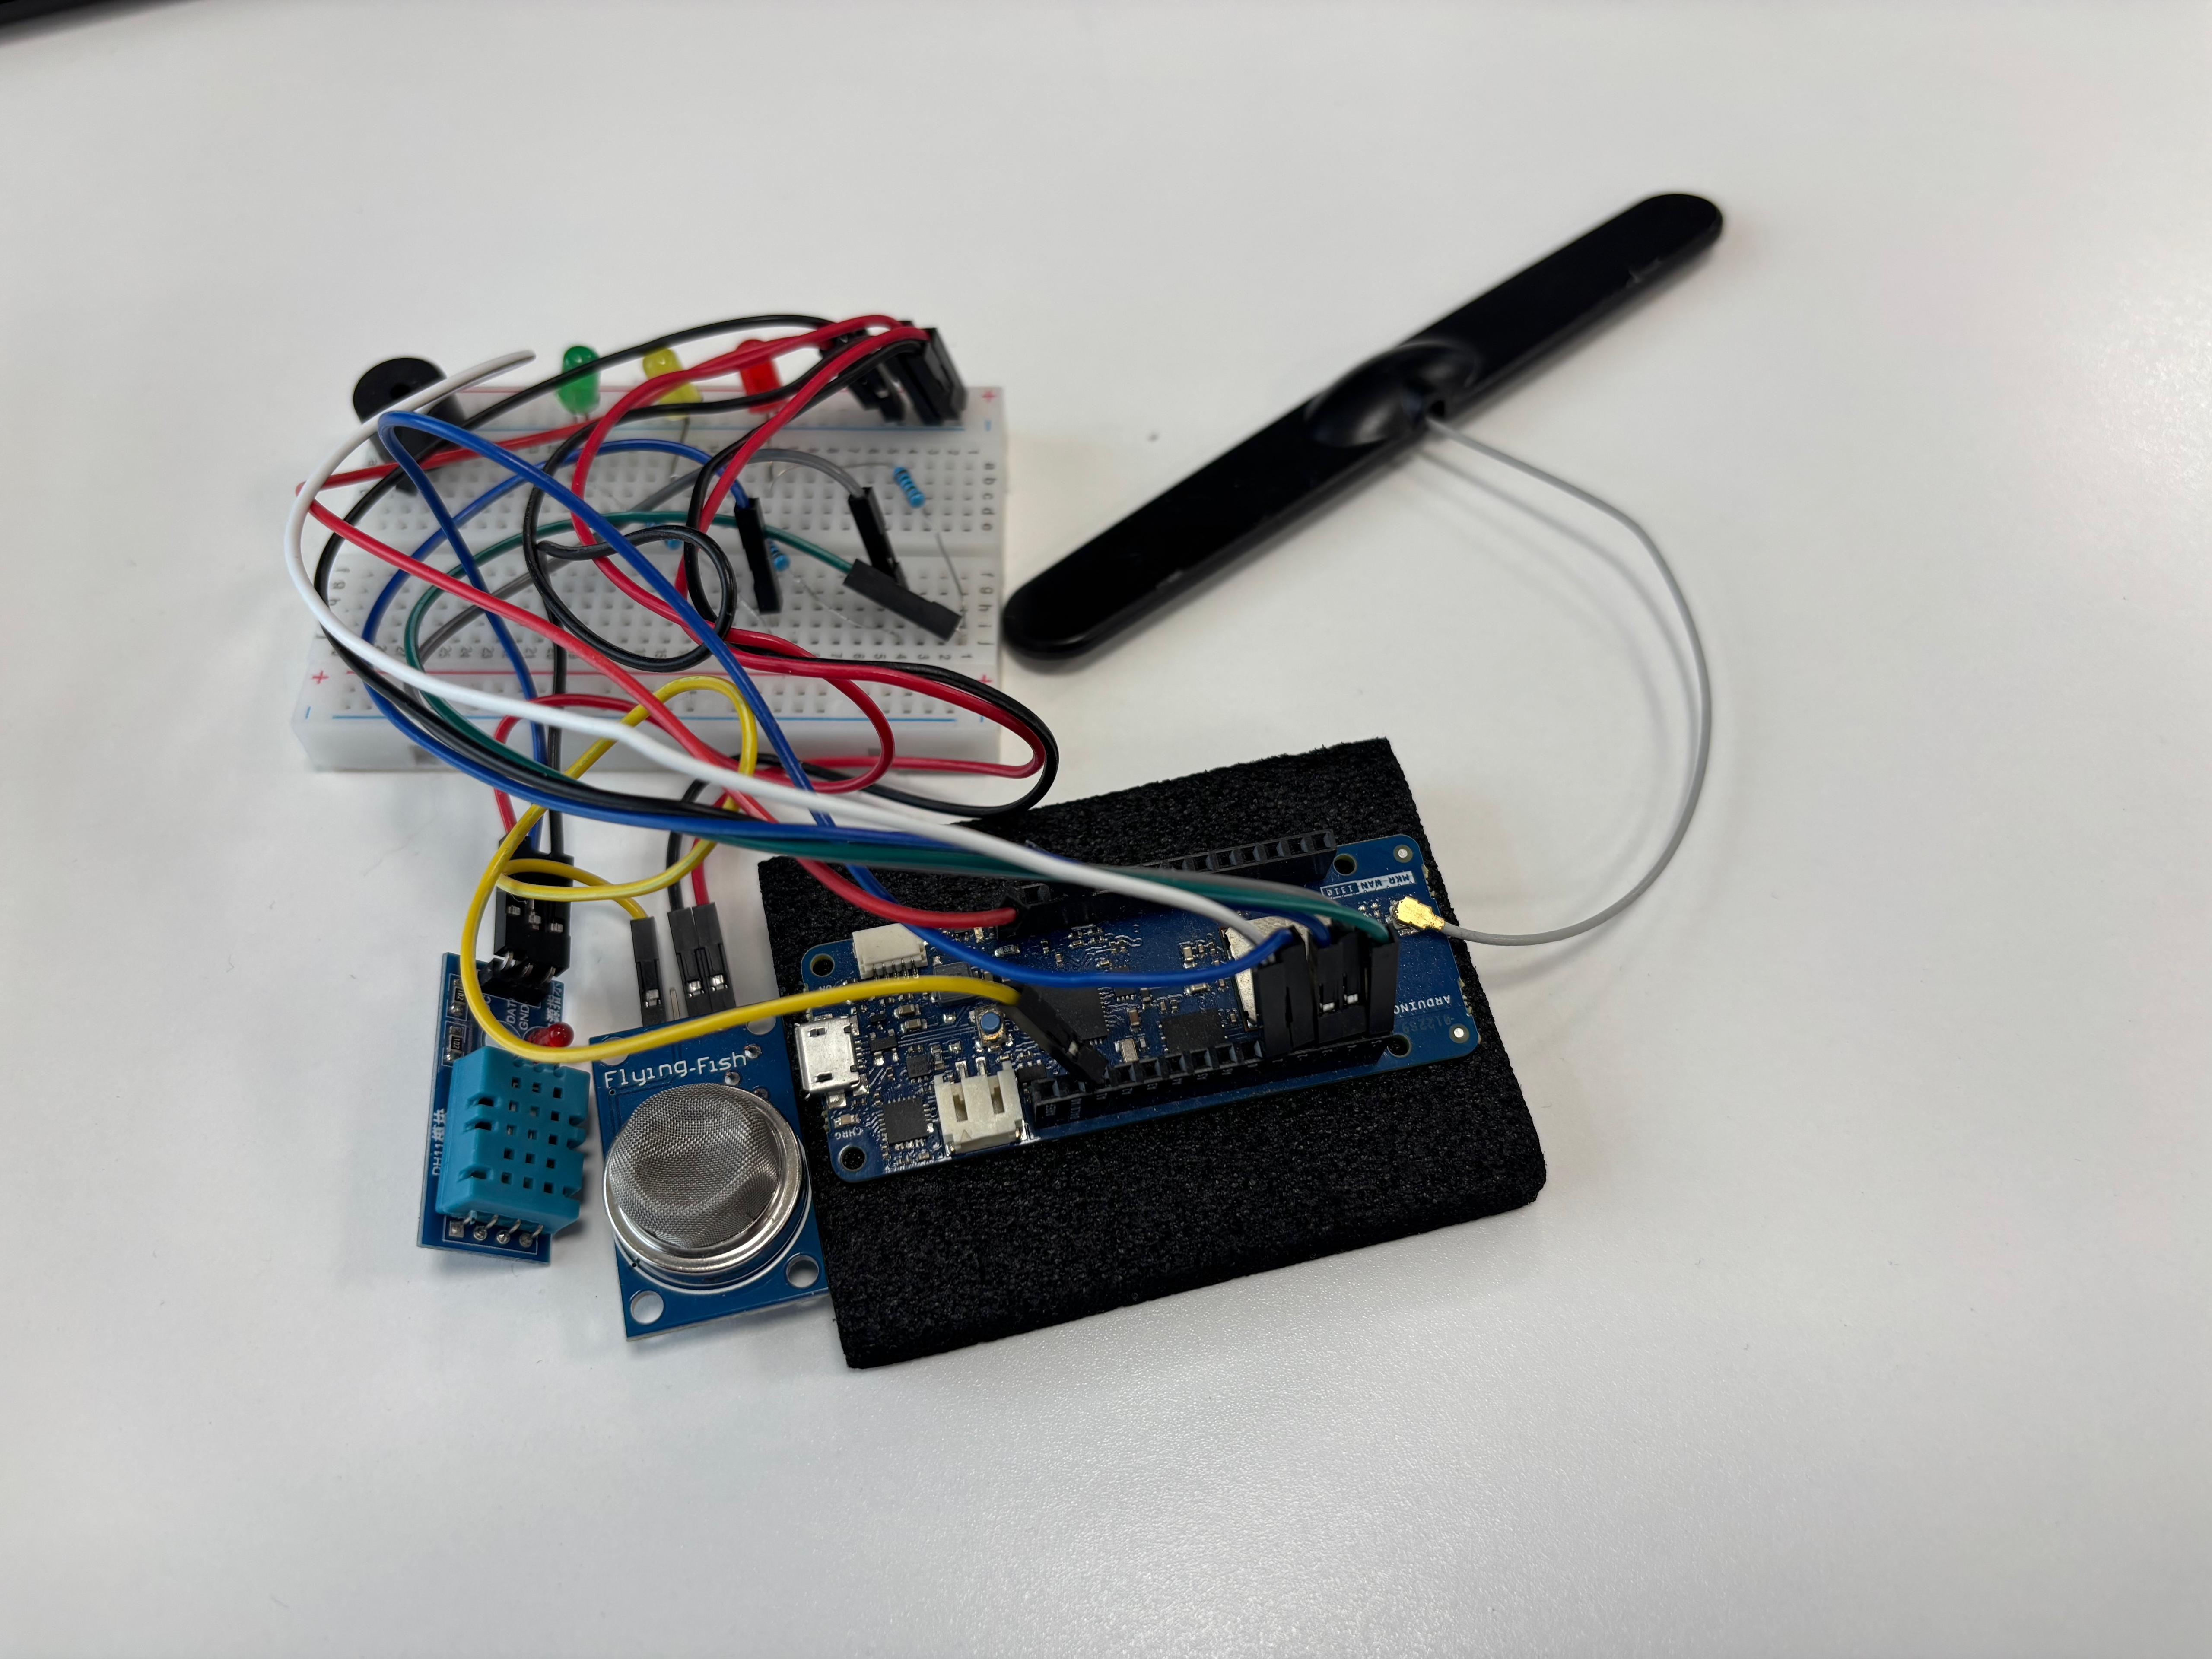
\includegraphics[width=0.7\textwidth]{Irudiak/sentsore_modulua.jpg}}
    {\fbox{\parbox[c][5cm]{0.8\textwidth}{\centering Irudia falta da: sentsore\_modulua.jpg}}}
    \caption{Sentsore modulua (Nodoa) bere osagaiekin: DHT11, MQ-135, bateria eta antena}
    \label{fig:sentsore_modulua}
\end{figure}

\begin{figure}[H]
    \centering
    \IfFileExists{Irudiak/modulu_zentrala.jpg}
    {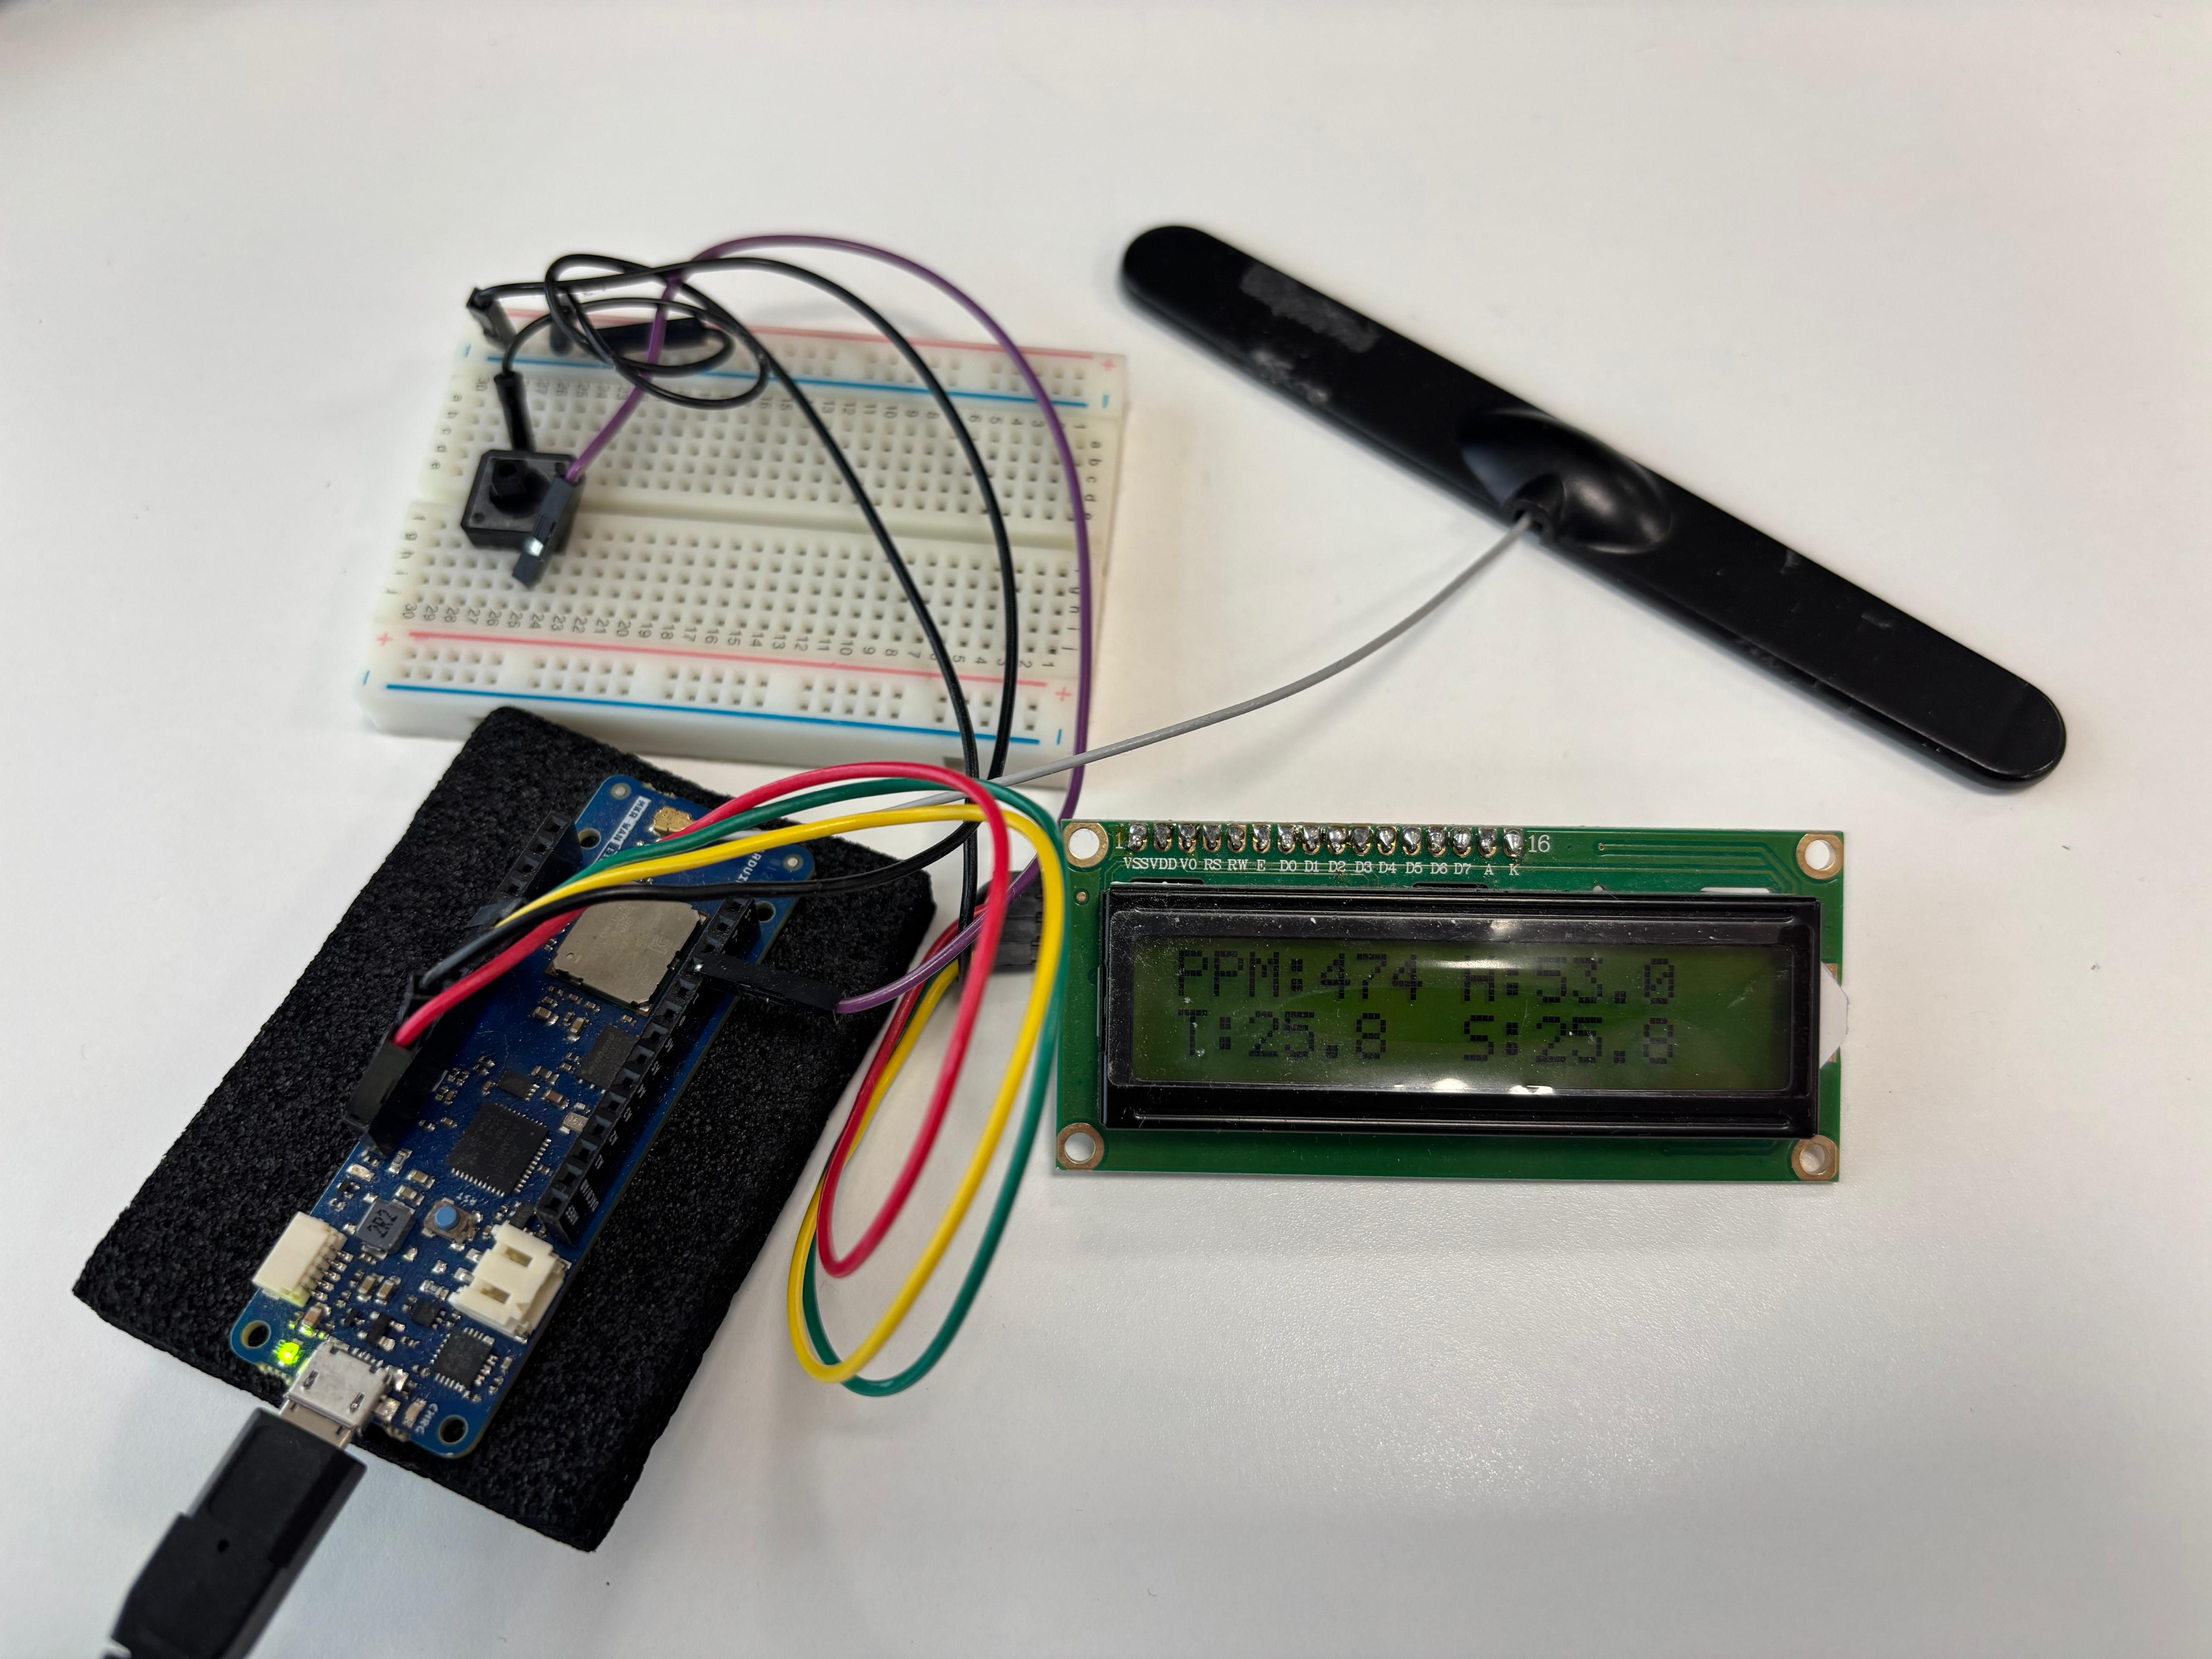
\includegraphics[width=0.7\textwidth]{Irudiak/modulu_zentrala.jpg}}
    {\fbox{\parbox[c][5cm]{0.8\textwidth}{\centering Irudia falta da: modulu\_zentrala.jpg}}}
    \caption{Modulu zentrala (Gateway) LCD pantailarekin datuak bistaratzen}
    \label{fig:modulu_zentrala}
\end{figure}
\vspace{0.5cm}

%\section{Sistema}

Gure proiektuaren osagai guztiak aipatu ondoren, osagai bakoitza banan-banan azalduko dugu. Gure sistemaren helburua airearen kalitatearekin lotutako datuak biltzea denez, bi sentsore mota inplementatuko ditugu gure nodoan:\\
\begin{itemize}
\label{sentsoreakje}
    \item \hyperlink{MQ}{\textbf{MQ-135}}: Sentsore hau airearen kalitatea aztertzeko erabiliko da. Hainbat substantzia toxikoren presentzia detekta dezake, hala nola, $NH_3$, $CO_2$, $NO_x$, bentzenoa edo kea, adibidez.\\
 
    \item \hyperlink{DHT}{\textbf{DHT11}}: Hau da gure sistemak erabiliko duen tenperatura eta hezetasun sentsorea. Tenperatura eta hezetasun sentsore konplexu bat dauka, gainera, seinale digitalaren irteera kalibratu batez hornituta. Seinale digitalak eskuratzeko teknika esklusiboa aplikatuz, eta, tenperatura eta hezetasuna detektatzeko teknologia erabiliz, fidagarritasun handia eta egonkortasun bikaina ziurtatzen ditu epe luzera. Sentsore honek hezetasuna neurtzeko osagai erresistibo bat eta tenperatura neurtzeko \ac{NTC} osagai bat ditu; eta, gainera, 8 biteko errendimendu handiko mikrokontrolagailu batera konektatzen da, kalitate bikaina, erantzun azkarra eta interferentzien aurkako gaitasuna eskainiz.\\

\end{itemize}

Lehen aipatu bezala [\ref{arduinomkr}], gure sistemak Arduino MKR WAN 1310 mikrokontrolagailu-plaka erabiliko du. Gure modulu bakoitzak esandako plaka bat izango du, eta, gure hardware-sistemaren nukleoa izango da. Plaka berezi hau micro-\ac{USB} kable batek elikatu ahal duen arren, bateria kargagarri batera ere konekta daiteke. Kasu honetan, modulu zentrala ordenagailura konektatuta egon behar denez, lehenengo tipoko konexioa erabiliko da. Urrutiko modulurako, edo beste era batera, sentsore modulurako, bateria kargagarriarena.\\

Gainera, gure modulu guztiek informazioa trukatuko dute modulu nagusiarekin; beraz, \ac{LoRa} komunikazio-teknologia erabiltzeko, modulu bakoitzak antena bat izango du zuzenean plakara konektatuta. MKR WAN 1310ek antena mota hori zuzenean konektatzeko leku berezi bat du. \\

Orain, falta zaizkigun osagaiak ondo ulertzeko, moduluak banan-banan aztertuko ditugu. Bi moduluak izango baitira gure sistema osatuko duten bloke nagusiak.\\

Lehenik, sentsore-nodo deitzen diogun modulua deskribatuko dugu. Bere funtzioak ondokoak izango dira: \\
\begin{itemize}
    \item Aurretik [\ref{sentsoreakje}] deskribatutako sentsoreen datuak biltzea.
    \item Airearen kalitate-mailak LED sistema baten bidez erakustea.
    \item Airearen kalitatea arriskutsua denean soinu-seinaleak igortzea.
    \item Datuak \ac{LoRa} bidez bidaltzea
\end{itemize}

\vspace{0.25cm}

LED bakoitzeko, erresistentzia eta PIN bana erabiliz, semaforo baten antzerako muntai erraz bat lortuko da. Semaforoko kolore bakoitzak ondoko esanahia izango du: \\

\vspace{0.15cm}

\begin{itemize}
    \item Berdea airearen kalitate onerako.
    \item Horia partikula kaltegarrien maila altuagoa detektatzen duenerako, $CO_2$a bereziki.
    \item Gorria aireztapena beharrezkoa denerako.
\end{itemize}

Zehazki, argi berdea 3.PINera konektatuta egongo da, horia 4.PINera, eta, gorria 5.PINera.\\

Soinu-jakinarazpenak lehenengo pin digitalera konektatutako active buzzer baten bidez transmititzen dira. \hyperlink{Buzz}{Active Buzzer}a gailu elektroakustiko bat da, eta, korronte elektriko bat bertatik igarotzen denean, soinu zorrotz eta entzungarri bat sortzen du. Normalean alertetarako erabiltzen da, gure kasuan bezala.\\

Sentsoreei buruz hitz eginez, DHT11 sentsorea bigarren pin digitalera konektatuta egongo da, eta MQ-135 sentsorea A1 pinera, lehenengo pin analogikora. Azken honek pin digital batera konektatzeko aukera duen arren, nahiago izan dugu irteera analogikoa erabiltzea, izan ere, modu honetara datu zehatzagoak lortzen ditu. Azkenengo kasu honetan, pin digitalak soilik esango liguke gasen kantitatea aurre ezarritakoa baino altuagoa edo baxuagoa den \cite{mq135_sensor}. Garrantzitsua da kontuan izatea bi sentsoreek 5 V-eko sarrera-seinalea behar dutela behar bezala funtzionatzeko. Horrenbestez, elikadura iturriak 5 V-eko pinera konektatu ditugu, eta ez $V_{cc}$ pinera. \\


Behin sentsore modulua deskribatuta, orain modulu zentrala azalduko da. Azken honek, sentsore-nodotik jasotako datuak erakutsiko dizkio erabiltzaileari \ac{LCD} pantaila baten bidez. \ac{LCD} pantaila batek oso konplexua ez dela ematen duen arren, kristal likidozko pantaila-sistemara konektatzea konplexua izan daiteke, azken hau kontrolatzeko interfazea 16 pinek osatzen baitute. Arduino plakaren eta \ac{LCD}aren arteko konexioak sinplifikatzeko, \ac{I2C} modulu bat sartu da. \\

% --- EXPLICACIÓN I2C Y SOLDADURA ---
Modulu hau erabiltzea ezinbestekoa izan da konexioak errazteko. Izan ere, jatorrizko \ac{LCD} pantailak 16 pin ditu, eta horiek guztiak kontrolatzeko kableatu oso konplexua behar da. \ac{I2C} egokigailuari esker, 16 pin horiek 4 pinera murrizten dira: \ac{SDA} eta \ac{SCL} (komunikaziorako), VCC (5V) eta GND (Lurra). Prozesu honetan lan manuala egin behar izan da, \ac{I2C} modulua pantailaren atzealdean zuzenean soldatu baitugu, 16 pinak banan-banan elkartuz konexio sendo eta iraunkor bat lortzeko.\\

Azkenengo honek konexioak asko sinplifikatzen ditu, eta, bere aplikaziorako, \ac{SDA} eta \ac{SCL} sarrerak baino ez dira behar 5 V-eko eta lurreko elikadurekin. Beraz, kontrolagailuak aginduak bidaliko ditu \ac{I2C} busaren bidez \ac{SDA} pina erabiliz. Beste lerroak serieko erloju-pin gisa funtzionatzen du (\ac{SCL}), eta Arduino plaka kontrolatzaileak tarte erregularretan bidaliko ditu seinaleak. Kasu honetan, Arduino MKR WAN plakak apropos prestatuta ditu 11 (\ac{SDA}) eta 12 (\ac{SCL}) pin digitalak \ac{I2C} moduluarekin (\hyperlink{\ac{I2C}}{I2C Protokoloa}) komunikatzeko.\\

Atal honekin amaitzeko, gure modulu nagusiak botoi bat izango du, eta, sakatuz gero, agindu bat bidaliko dio sentsore-nodoari, LEDez osatutako semaforoa pizteko edo itzaltzeko. Pin digitala pull-up sarrera gisa definituko da. Horrenbestez, botoia sakatzerako orduan, 0ko balioa itzuliko du lurrera konektatuta dagoelako.\\

\subsubsection{Sentsoreak}

Aurreko atalean [\ref{arduinomkr}] erbilitako materiala eta muntaia azaltzerako orduan, sentsore modulua osatzen duten sentsoreak aipatu dira, DHT11 eta MQ-135 sentsoreak hain zuzen ere. Helburuetan [\ref{sec:faseak}] argi ikusi da atal honen garrantzia, izan ere, sentsore bakoitza mundu bat den heinean, sentsoreen datuak ulertzea eta prozesatzea ezinbestekoa da. Lehen aipatu bezala, sentsoreak arduino plakara konektatzea lortu dugu konexio egokiekin. Beraz, puntu honetara iritsita, sentsoreek bidaltzen duten informazioa eskuratzea izango da hurrengo urratsa.\\

Sentsoreen datu prozesaketarekin hasteko, interesgarria da sentsoreen kalibrazioari erreparatzea. Alde batetik, DHT11 sentsorea daukagu. Datu-orrian irakur dezakegunez (\hyperlink {DHT} {DHT11 Datasheet}), sentsoreak tenperaturari eta hezetasunari buruzko datuak dituen 40 biteko seinale bat itzuliko du. Gainera, seinaleari buruz nahi ditugun datuak lortzeko \hyperlink {DHT} {Adafruiten DHT sentsorearen liburutegia} erabiltzen da. Liburutegi hori programan sartuz,\textit {''dht.readHumidity()''} eta \textit{''dht.readTemperature()''} funtzioak erabil daitezke, zenbaki erreal gisa hezetasun erlatiboa eta tenperatura itzuliko dituzten funtzioak hain zuzen ere. Gainera,\textit {''dht.computeHeatIndex(t, h, false)''} kodea erabiliz, non t tenperatura den, h \ac{RH}a den, eta ''false''k emaitza Celsiusetan nahi dela adierazten duen, bero-indizea zuzenean lortzen da kalkulu gehigarririk egin gabe.\\

Beste alde batetik, MQ-135 sentsorearen kalibrazioa pixka bat konplikatuagoa da. Izan ere, airearen kalitatea ezagutzen den eremu kontrolatuetan esperimentatzeko ekipoa ez edukitzeak zaildu egiten du sentsorearen kalibrazio optimoa. Beraz, gure kalibrazioa esperimentuetan lortutako emaitzekin osatuko da. Gainera, gomendagarria da elikatze-iturria sentsore-nodotik ahalik eta gutxien deskonektatzea. Horren arrazoia MQ sentsoreak aurreberotze-denbora oso luzea duela (24 ordu baino gehiago) da, eta, beraz, sentsoreen modulua etengabe itzaltzen eta pizten badugu, denbora asko itxaron beharko dugu airearen kalitatearen neurketa onak lortzeko.\\

\subsection{LoRa}
\label{sec:lora}

\subsubsection{LoRa protokoloa}
\label{protocollora}

\ac{LoRa} \ac{CSS} modulazio teknologia erabiltzen duen hari gabeko teknologia da, Semtech izeneko fabrikatzaileak patentatutakoa. Gure aplikaziorako oso egokia da, izan ere distantzia handiekin lan egiteko eta aipatutako [\ref{fig:muntaia}] \ac{IoT} sareak eraikitzeko gai da (bereziki sentsore sareak).

\ac{LoRaWAN}-ekin alderatuz desberdintasun nabariak ditu.
Azkenengo hau \ac{LoRa} dispositiboak komunikatzeko eta antolatzeko erabiltzen den sare protokolo bat baita. Potentzia baxuko sareetan aplikatzeko oso egokia da, eta eremu zabaletan lan egiteko gaitasuna dauka \cite{moya2018evaluacion}.

\ac{LoRaWAN} sare oso baten eskema orokor bat ikus daiteke \ref{fig:muntaialor}.irudian. Irudikatutako eskemarekin [\ref{fig:muntaia}] alderatuz, bertan agertzen diren nodo amaierak, gure sentsore moduluak izango lirateke.\\
Gateway-a edo Sare-Sarbidea, aldiz, modulu zentrala izango litzateke, zeinak nodo amaieren datuak jasoko dituen.\\
Agertzen diren gainontzeko elementu guztiak \ac{LoRaWAN} sare zabalago batentzako izango lirateke, eta ez dira erabiliko gure sarean.\\

\begin{figure}[!htbp]
    \centering
    % Control de errores para imagen
    \IfFileExists{Irudiak/lorawan_network_architecture.png}
    {\includegraphics[width=\textwidth]{Irudiak/lorawan_network_architecture.png}}
    {\fbox{Irudia falta da: lorawan\_network\_architecture.png}}
    \caption{LoRaWAN sarea}
    \label{fig:muntaialor}
\end{figure}

\ac{LoRa}k erabiltzen duen modulazio teknika dela medio, hartzaileek sentsibilitate altuagoa izatea ahalbidetzen du. Gainera, gehiengo irrati-sistemekin alderatuz, \ac{LoRa} irratiek 10 aldiz ahulagoak diren seinaleak jasotzeko gaitasuna daukate. Aipatutakoa ulertzeko, potentziaren aldaketa batek zelan eragiten duen kasu bakoitzean aztertuko da.\\

Irrati-sistema konbentzionaletan igorlearen potentzia 10 alditan handituz gero, hartzailearen komunikazio helmuga proportzinalki handitzea edo hartzailearen sentsibilitatea 10 alditan hobetzea suposatzen du. 
Aldiz, \ac{LoRa} sistemen kasuan kontsumitutako potentzia edo igorlearen potentzia ez da handitu behar komunikazio tarte handi bat lortzeko \cite{bor2016lora}.\\

Atal honen hasieran [\ref{protocollora}] esan bezala \ac{LoRa}k \ac{CSS} modulazioa erabiltzen du. Aipatutako modulazio mota banda zabalerako teknika bat da, zeinak seinalea kodifikatzeko \textit{Chirp} \cite{springer2000spread} izeneko pultsuak erabiltzen dituen. Artikuluan ikusi daitekeen moduan, \textit{Chirp}ak seinale sinusoidalak dira, zeinen maiztasuna handitzen edo txikitzen den denboran zehar.\\

Atal honekin amaitzeko, \ac{CSS} modulazioa erabiltzearen zergaitia azalduko da. Izan ere, potentzia txiki, distantzia handi eta data ratio txikia eskatzen duten aplikazioetan erabiltzen da. Are gehiago, potentzia baxuetan lan egin arren, oso sendoa da zarataren eta Doppler efektuaren aurrean, energia txikiak eta uhin-zabalera handiak erabiltzen baitira oztopoak saihesteko \cite{chen2019micro}.\\

Beraz, aurreko guztia kontuan hartuta, ondorioztatu daiteke oso protokolo egokia dela diseinatuko sarerako.\\

\subsubsection{LoRa komunikazioa}

\ac{LoRa} izenak berak esaten duen moduan, \textit{Long Range} izateak irismen luzeko haririk gabeko sarearen teknika bat dela esan nahi du. Hiru maiztasun-bandatan lan eginez (433MHz, 868MHz, 915MHz), irrati-maiztasuneko seinaleak deskodetzen dira eta datuak trukatzen dira. \ac{LoRa} teknika segurua eta transmisiorako irismen handikoa da. Wi-Fi eta Bluetooth ez bezala, denbora luzeagoan bidal ditzakezu datuak, eta, horrek, bateria gutxiago kontsumitzea esan nahi du.\\

\ac{LoRa} erabiltzeko, \hyperlink {MKR} {Arduino MKR WAN 1310} plakak erabiliko ditugu gure sistema eraikitzeko. Plaka horiek ezin hobeak dira gure proiektua inplementatzeko, \ac{LoRa}ren bidez elkarrekin konektatzeko berariaz prestatuta daudelako. Azpiatal honetan, proposatutako sistemaren eragiketa-gaitasunak eta mugak eztabaidatuko dira. Bere gaitasun nagusietako bat gure plaken bi noranzkoko konexioa da. Plakak informazioa jasotzeko nahiz bidaltzeko gai dira, eta komunikazio-kanal oso erabilgarria ahalbidetzen dute.\\

Bestalde, gure ideia ezartzean aurkitu dugun mugarik handiena ere komunikazio-kanala da. Arazoa da, noranzko biko sistema denez, kanala gainkarga daitekela eta gure sistema blokeatu. Horregatik, gure sistemak ezin ditu sentsoreetatik datu jarraituak bidali. Saturazio hori konpontzeko, gure sentsore nodoa programatu dugu informazioa bidaltzeko hamar segundo inguruko atzerapenarekin. Hala ere, denbora-tarte horrek txikia izaten jarraitzen du, eta sistemak ondo funtziona dezake.\\

Gainera, aipatu behar dugu gure modulu nagusian semaforoa sentsore-moduluetan pizteko botoia erabiltzeak datu-igorpenaren arteko denbora-tartea handiagoa izatea eragin dezakeela. Izan ere, kasu honetan, nodoa informazioa aldi berean jasotzera eta bidaltzera behartzen ari gara.\\

Aipatu behar den azken gauza da \hyperlink {MKR} {Arduino MKR WAN 1310} delakoaren aukera zergatik den hain aproposa. Lehenik eta behin, oso egokiak dira \ac{LoRa} konektibitatea erabiltzeko, eta, bigarrenik, tamaina txikia (25mm x 67.6mm) abantaila bat da erabiltzailearentzat modulu txikiagoak eta eramangarriagoak sortzeko.\\

\vspace{0.35cm}

\section{Gauzen Interneta}

Gauzen Internet-a edo \acf{IoT} izatez komunikazio kontzeptu bat da, zeinean objektu fisiko edo gailu multzo bat interkonektatuta dagoen, esate baterako Wi-fi eta Bluetooth-aren kasuan gertatzen den moduan. Gaur egun, pil-pilean dagoen kontzeptu bat da, izan ere mota askotako aplikazioak eskeintzen ditu bai industria eremuan baita eguneroko bizitzan ere; are gehiago, aplikazio horiek erabilgarriak dira automatizazioan, gizaki-makina komunikazioan, jasangarritasunean, eraginkortasunean eta segurtasunean.\\

\begin{figure}[!htbp]
    \centering
    % Control de errores para imagen
    \IfFileExists{Irudiak/IoT_GrAL.png}
    {
\includegraphics[width=\textwidth]{Irudiak/IoT_GrAL.png}}
    {\fbox{Irudia falta da: IoT\_GrAL.png}}
    \caption{IoT kontzeptuaren eskema orokorra}
    \label{fig:muntaiaiot}
\end{figure}

Esan bezala, gailu edota objektu fisikoen artean beharrezko konexioak egiteko, \ac{IoT}k datuak bildu, prozesatu eta sare bat erabiliz bidaltzeko gaitasuna izan behar du. Sarearen bidez informazioa bidali ostean, datuak manipulatzeko aukera ere izan dezake. Teknologia hau oso zabala eta malgua den heinean, hainbat konbinazio mota eskeiniko ditu, zeinak era zorrotz batean egokitu diren nahi dugun aplikazioa burutzeko.\\

\ac{IoT} sare bat eraikitzerakoan erabiliko den komunikazio protokoloak berebiziko garrantzia izango du, alegia, hainbat gailu komunikatzeko erabiliko den teknologia ulertzea ezinbestekoa da. Mota askotako protokoloak existitzen dira, hainbat aplikazio desberdinetan erabiltzeko, eta, honekin batera, badaude \ac{IoT}-rako komunikazio protokolo zehatzak edo \ac{IoT}-n erabili daitezkenak. Orokorrean, makinatik makinarako protokoloak dira, \ac{M2M}. Beraz, elkar komunikatzeko gai diren gutxienez bi gailuk konposatutako sistema bat osatuko dute.\\

Atal honetako helburua sentsoreen bidez jasotako datuak zuzenean InfluxDB datu-base espezifiko batera pasatzea da. InfluxDB-k bere web orria dauka, eta, bertan, jasotako datu guztiak zuzenean ikus daitezke monitorizazioa eta azterketa errazteko. Linux ingurunean exekutatuko diren hiru zerbitzariak Docker bidez izango dira. Docker zerbitzu bakoitzeko ataka bat izango dugu, zeintzuk zerbitzuen arteko komunikazioa ahalbidetuko duten.\\

\subsection{IoT ataleko Muntaia eta Osagaiak}

Sare eraikitzen atalean gure egituraren eskema orokor bat ikus dezakegu \ref{fig:muntaia}. irudian. Atal horretan eskemako osagai guztiak landu ditugu \ac{IoT}-ko atala kenduta. Orain arte, oso era laburrean esanda, sentsoreetako datuak ordenagailura pasatu dira, eta, puntu honetan, ordenagailutik influx DB izeneko datu-base batera pasa behar ditugu ordenagailuan jasotako datuak \ac{IoT} tresna batzuk erabilita. Ordenagailutik  datu-basera arteko prozedura hobeto ulertzeko, ondoko irudia dago \ac{IoT}-ko prozedura guztiekin.\\

\begin{figure}[!htbp]
    \centering
    % Control de errores para imagen
    \IfFileExists{Irudiak/IoT_muntaia.png}
    {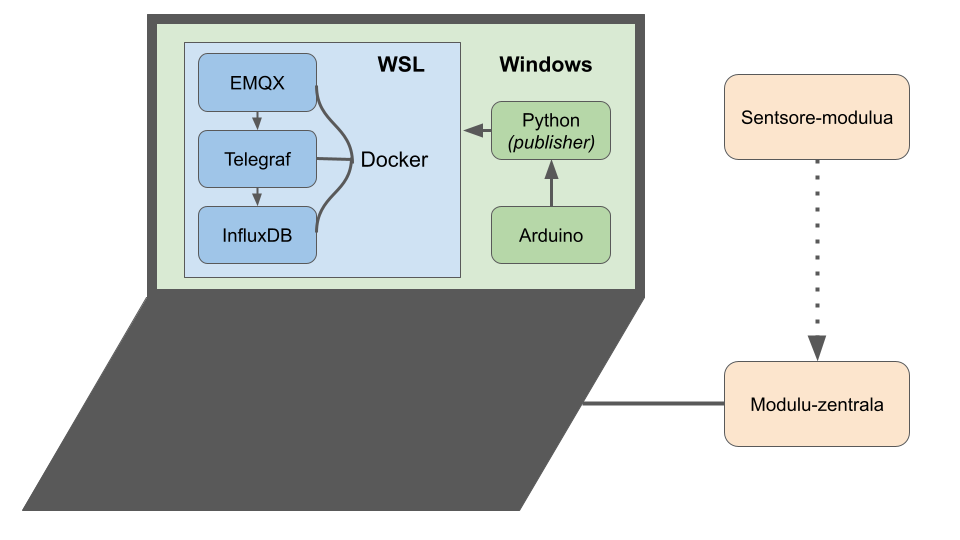
\includegraphics[width=\textwidth]{Irudiak/IoT_muntaia.png}}
    {\fbox{Irudia falta da: IoT\_muntaia.png}}
    \caption{IoT-ko muntaia}
    \label{fig:iotmuntaia}
\end{figure}

Badakigunez, sentsore-moduluko datuak modulu zentrala bidaliko dira hari gabeko \ac{LoRa} teknologia erabiliz. Modulu zentrala ordenagailura konektatuta egongo da, eta, bertan, arduinoko programaren bidez datuak igorriko dira.\\

Hemendik aurrerako osagaiak orain arte ezezagunak dira, eta, banan-banan azalduko dira ordenagailutik datu-baserako bidea osatzen dituzten elementuak; haien funtzionamendua eta garrantzia proiektu honetan hobeto ulertu ahal izateko.\\

\ac{IoT} sare bat eraikitzeko teknologia ez da bakarra eta hainbat baliabide aurki daitezke beharren arabera. Hala ere, kasu honetan, tresna orokor batzuk aplikatu dira, zeintzuk komunikazio protokolo zehatz batekin erabili diren, \ac{MQTT} protokoloarekin hain zuzen ere.\\

\subsubsection{\ac{MQTT} protokoloa}

Aipatu bezala, mota askotako komunikazio protokoloak daude eta haien arteko bateragarritasuna ez dago beti bermatuta. Egon daitezkeen bateragarritasun arazoak ekiditeko, \ac{MQTT} protokolo estandar eta irekia daukagu. 
Kasu honetan, \ac{M2M} protokolo batekin lan egiten da, zeinak \textit{PubSub} metodologia erabiltzen duen \textit{Message Queue} komunikazioa erabiliz \cite{hunkeler2008mqtt}.\\

Beraz, esandako guztiarengatik eta protokolo sinple eta erabilgarria delako, \ac{MQTT} erabiliko da komunikazio protokolo gisa.\\

\begin{figure}[!htbp]
    \centering
    % Control de errores para imagen
    \IfFileExists{Irudiak/MQTT_irudia.png}
    {\includegraphics[width=\textwidth]{Irudiak/MQTT_irudia.png}}
    {\fbox{Irudia falta da: MQTT\_irudia.png}}
    \caption{MQTT komunikazio-protokoloa}
    \label{fig:mqttirudia}
\end{figure}

\ac{MQTT} protokoloa broker bideratzaile batean oinarritzen da: mezu bakoitzak \textit{topic} edo gai bat darama, eta mezua argitaratzen duen bezeroak erabakitzen du zein den gaia. Bezeroa \textit{topic} jakin bati harpidetzen bada, \textit{broker}-ak gai horri dagozkion mezu guztiak bidaliko dizkio. Gainera, mezuak ilara batean gordetzen dira, bezeroak jaso arte galdu ez daitezen; hori da \textit{Message Queue} azpiegituraren oinarria.\\

\ref{fig:mqttirudia}.irudiko adibidean, \textit{topic}-a \textit{tenperatura} da, eta, tenperatura-sentsoreak datuak argitaratzen ditu gai horrekin. Kasu honetan, gainera, bezeroek ordenagailu edo mugikor baten mezuak jasoko dituzte.\\

Protokoloa inplementatzeko, Python programazio-lengoaia eta EMQX izeneko \textit{broker}-a erabiliko dira, Docker bidez inplementatuta, zeintzuk jarraian azalduko diren.\\

\subsubsection{Python}
Windows sistema eragilean, Arduino programaz gain, Python erabiliko dela ikus daiteke \ref{fig:iotmuntaia}.irudian. Graduan zehar ikusi bezala, jakin badakigu zer motatako kodea den Python, oso erabilgarria izango dena testuinguru honetan. Python lenguaia erabiltzeko, doako Spyder \ac{IDE}a erabiliko da, zeina iturri irekikoa \textit{(open source)} den. Orokorrean zientzialari, ingeniari eta datu analistentzako bideratuta dagoenez, ingurumen zientifiko batean lantzen da.\\

\subsubsection{WSL}

Linuxen erabiliko ditugun aplikazio desberdinak zabaltzeko Docker erabiltzen da. EMQX, Telegraf eta Influx DB zabaltzeko hain zuzen ere. 
Docker-a software modularra eta iturburu irekiko plataforma da, zeinaren funtzio nagusia aplikazioak modu eraginkorrean zabaltzea, mantentzea eta hedatzea den. Makina birtualekin alderatuta, Docker-ak \textit{host}-aren sistema eragilea erabiltzen du, errendimendu hobea eta baliabideen optimizazioa lortuz \cite{microsoft_wsl}. Gainera, hainbat \textit{container} aldi berean exekutatzeko gai izango da abiadura eta memoria erabilera baxua mantenduz.\\

Docker-ek \textit{container} birtualak erabiltzen dituzte aplikazioak isolatzeko eta exekutatzeko. \textit{Container} bakoitzak bere barnean edukiko ditu aplikazioaren kodea eta beharrezko osagai guztiak, edozein ingurunetan modu fidagarrian exekutatu ahal izateko. Modu honetan, aplikazioak eramangarriagoak izango dira eta edozein sistema eragile agnostikotan exekutatu ahal izango dira, ingurune jakin batekiko bateragarritasun arazoak saihestuz. Hala ere, kasu honetan erabili den ordenagailua Windows sistema eragilearekin erabili denez, eta Dockerraren funtzionamendua hobea denez Linux-en aurrean, \ac{WSL} erabili da. Izan ere, Linuxeko \textit{kernel}a erabiltzen du eta \textit{container}-ak modu arinago eta eraginkorragoan exekutatzeko baliabide hobeak ditu \cite{merkel2014docker}. \\

\begin{figure}[!htbp]
    \centering
    % Control de errores para imagen
    \IfFileExists{Irudiak/Docker_Architecture.png}
    {\includegraphics[width=\textwidth]{Irudiak/Docker_Architecture.png}}
    {\fbox{Irudia falta da: Docker\_Architecture.png}}
    \caption{Docker-aren arkitektura}
    \label{fig:docker_architecture} 
\end{figure}

Docker-aren funtzionamendua hobeto ulertzeko, Docker irudia \textit{(image)} zer den ulertu beharra dago. Docker irudia aplikazio bat exekutatzeko beharrezko fitxategi eta konfigurazio guztia dituen txantiloi bat da, zeina oinarri moduan erabiltzen den \textit{container} bat sortzeko. \textit{Container}-a, aldiz, irudi horren exekuzio-instantzia bat da; hots, Docker irudia erabiliz sortutako aplikazio isolatua eta exekutagarria.\\

Software modularra erabiltzeko, Docker Hub webgunean hainbat irudi aurki daitezke, deskargai eta erabilgarri. Irudi horiek gure beharrak ez balituzte beteko, erabiltzaileak bere irudi propioak sor ditzake. Kasu honetan, teknologia honen muina Docker Engine den arren, eraiki nahi den sarerako Docker Desktop erabiliko da. Docker Desktop-ak \textit{container} eta irudien kudeaketa erraztu eta bezero-zerbitzari egitura jarraitzen duelako: Bezeroak \textit{(client)} zerbitzariari \textit{(daemon)} aginduak bidaltzen dizkio, eta, biak makina berean edo urruneko zerbitzari batean egon daitezke ondoko irudian ikusi ahal den moduan. \\

Bere exekuziorako terminalean komando bakar batekin \textit{(docker run ...)} irudi bat deskargatu, eta, hortik \textit{container} berri bat sor daiteke, aplikazioa martxan jarriz. Izan ere, lehenengo aldiz irudi bat exekutatzen denean, \textit{container} bat sortzen da automatikoki; horrela, aplikazio bat martxan jarriz erabiltzailearen makinan. Beraz, aurretik aipatutako hiru aplikazioak erabiltzeko, haien Docker irudiak lortu eta aplikazio bana sortuko da. Horrela, soilik \textit{container}-ak exekutatuz, aplikazioak arazorik gabe erabili ahalko dira. \\

\subsubsection{EMQX}

Dockerra zer den ulertuta, EMQX zer den jakin dezakegu. EMQX \ac{MQTT} broker bat da; hau da, \ac{MQTT} protokoloan oinarritutako zerbitzaria, gailu ezberdinen arteko mezuak kudeatzen eta bideratzen dituena. Gure kasu partikularrean \ac{IoT}-eko aplikazio honetan mezulari lana egingo du. \\

Lehen aipatu bezala, Influx DB-ra informazioa bidaltzeko beste edozein aplikazio erabil zitekeen arren, proiektu honetarako hau erabili da hainbat arrazoiengatik. Hasteko, gailuen konektibitatea bermatzen du, eta, kasu honetan, sentsoreen balioen transmisioa bermatuko du. \ac{MQTT} protokoloa erabiltzen du proiektuko atal honetako \ac{IoT}-eko aplikazio guztien moduan, mezuen entregaren fidagarritasuna ziurtatuz. \\

Gainera, oso interesgarria den puntu bat eskalagarritasuna da; hots, gailu gehiagoren beharrei erantzuteko gai da. Azken hau gure sare malguarentzako oso beharrezkoa den ezaugarri bat izango da. Azkenik, segurtasuna aplikazio honen beste puntu garrantzitsu bat izango da, izan ere, autentifikazioa, segurtasuna eta datuen enkriptazioa eskaintzen ditu \cite{bender2021open}. \\

\begin{figure}[!htbp]
    \centering
    % Control de errores para imagen
    \IfFileExists{Irudiak/emqx_eskema.png}
    {\includegraphics[width=\textwidth]{Irudiak/emqx_eskema.png}}
    {\fbox{Irudia falta da: emqx\_eskema.png}}
    \caption{EMQX brokerraren eskema}
    \label{fig:emqxirudia}
\end{figure}

\ref{fig:emqxirudia}.irudian ikus daitekeen moduan, EMQX eskemaren zentruan egongo da, eta, berari konektatuta gutxienez \textit{publisher} eta \textit{suscriber} bana egongo dira. Hala ere, aurretik aipatu bezala, \textit{publisher} eta \textit{suscriber}-en kopurua malgua da.\\

Kasu honetan, \textit{publisher}-a Pythonen egindako programa izango da, zeinak arduinon jasotako mezuak bidaliko dituen. Ondoren, EMQX izango dugu, mezuak \ac{MQTT} protokoloan izateko. Azkenik, Telegraf deitzen den \textit{suscriber}-a izango dugu, zeinak bitartekari gisa lan egingo duen gure azkeneko helburua lortzeko, datuak InfluxDB-ra bidaltzea.\\

\subsubsection{Telegraf}

\ac{MQTT} protokoloa InfluxDB-rekin konektatzeko zubi gisa Telegraf erabiliko da. Telegraf iturburu irekiko datu-bilketa ordezkari \textit{(agent)} bat da. Gure \ac{IoT} egituran, Telegrafek \ac{MQTT}-tik edo beste datu-iturri batetik datuak jasoko ditu, eta, prozesaketa orokorra egiteko aukerak eskainiko ditu. Azkenik, datuak InfluxDB-ra bidaliko ditu, bertan informazioa modu eraginkorragoan adierazteko.\\


\ref{fig:telegrafirudia}.irudian ikus daiteken moduan,
Telegraf-en funtzionamenduaren eskema orokorra dago, zeinak lau atal nagusi dituen. Lehenengoa, datu-sarrerari dagokio, eta, Telegrafek ehunka datu-iturrirekin funtzionatzeko aukera ematen du. Iturburu irekiko tresna izanik, erabiltzaileek nahi duten datu-iturria gehitzeko aukera daukate, beti ere jadanik integratuta ez badago. Gure kasuan, ez da aldaketarik egin behar izan, \ac{MQTT} intrintsekoki erabilgarri daukalako. \\

Horrez gain, prozesatzaileak daude, zeintzuk datuak eraldatu, iragazi edo apaindu ditzaketen. Gauzak horrela, datuak InfluxDB-n gordetzea errazten eta sinplifikatzen da.  Hori gutxi izan balitz, eransgailuak ditugu, eta, hauek datuen batezbestekoa edo muturreko balioak aurrez kalkulatzeko erabiltzen dira, berriz ere datu-basean kudeaketa errazteko.\\

Azkenik, datu-irteerak daude. Hauek hainbat datu-basetara bidali daitezke, ez soilik InfluxDB hodeira \textit{(cloud)}.\\

\begin{figure}[!htbp]
    \centering
    % Control de errores para imagen
    \IfFileExists{Irudiak/telegraf_irudia.png}
    {\includegraphics[width=\textwidth]{Irudiak/telegraf_irudia.png}}
    {\fbox{Irudia falta da: telegraf\_irudia.png}}
    \caption{Telegrafen funtzionamenduaren eskema orokorra}
    \label{fig:telegrafirudia}
\end{figure}

\subsubsection{Influx DB}

Python eta \ac{MQTT} protokoloaren bidez lortuko da datuak nodo batetik zentrora \textit{(gateway)} bidaltzea, eta, ondoren, zerbitzari \textit{(broker)} batera eramatea. Azkenengo honek mezu eta datu guztiak kudeatuko ditu.  Hala ere, zerbitzariak ez ditu datuak gordetzen, eta, horretarako, datu-base bat beharrezkoa da. Aukeratutako datu-basea InfluxDB da, doakoa eta iturburu irekikoa dena. Oso egokia da denboran zehar aldatzen diren magnitudeak gordetzeko \cite{naqvi2017time}.\\

Gure kasuan, sentsoreak erabiliko direnez, hainbat parametro neurtuko dira, eta, hauen aldaketak denboran zehar bildu nahi direnez, InfluxDB oso egokia izango da. Datuak jasotzeaz eta biltzeaz gain, azkartasun handia bermatzen du denborarekin aldatzen diren datuak prozesatzeko. Gainera, aukera ematen du datuak modu ezberdinetan adierazteko eta ebaluatzeko. Esaterako, bi toki desberdinetan hartutako tenperaturak alderatu eta hauen batezbestekoa kalkulatzeko gai da. Horrez gain, hainbat motatako grafikoak erabil daitezke, datuen arabera adierazpen egokiena aukeratzeko.\\

\begin{figure}[!htbp]
    \centering
    % Control de errores para imagen
    \IfFileExists{Irudiak/influxdatanirea.png}
    {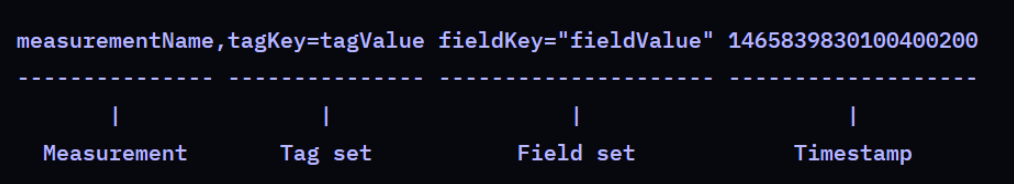
\includegraphics[width=\textwidth]{Irudiak/influxdatanirea.png}}
    {\fbox{Irudia falta da: influxdatanirea.png}}
    \caption{Influx DB-ko datuen egitura orokorra}
    \label{fig:influxegitura}
\end{figure}

Bestalde, InfluxDB-n datuak gordetzeko sintaxi zehatz bat erabiltzen da \cite{calabuig2022desarrollo}, eta, eskema bat ikus daiteke \ref{fig:influxegitura}.irudian.\\

Datu-egiturak lau elementu mota izango ditu. Lehenengoa, neurketaren izena da \textit{(Measurement)}, eta karaktere-kate \textit{(String)} gisa adierazi behar da, neurketa bakoitzeko izen bakarra izanik. Honen ondoren, koma bat jarri behar da, hutsunerik gabe. Bigarrenik, etiketak daude \textit{(Tag Key eta Tag Value)}, nahiz eta hauek hautazkoak izan. Etiketak karaktere-kateak dira, eta hainbat etiketa erabil daitezke, koma bidez bereizita.\\

Hirugarrenik, eremuak \textit{(Field Key eta Field Value)} daude. Gutxienez eremu bat adierazi behar da, nahitaezkoa baita. Eremuaren giltzak neurtzen den parametroaren izena adierazten du, eta, balioak parametro horren neurketa gordetzen du. Eremuak aurreko elementutik hutsune batez bereizten dira, eta, beste eremu batzuk gehitu nahi badira, koma batez banandu behar dira, nahi beste gehituz. Giltza karaktere-kate bat izan behar da, eta, balioa karaktere-katea, zenbaki osoa edo balio boolearra izan daiteke. Karaktere-katea bada, komatxoen artean idatzi behar da.\\

Azkenik, denbora-zigilua \textit{(Timestamp)} adieraz daiteke, baina ez da nahitaezkoa; jarri ezean, datu-baseak automatikoki esleituko du. Adierazi nahi izanez gero, \textit{Unix timestamp} motako datua izan behar da, eta eremuetatik hutsune batez bereizita egon behar da.\\

\subsection{Ordenagailutik Datu-Basera: Inplementazio Praktikoa}

Behin osagai teorikoak eta haien funtzioak azalduta, atal honetan sistema osoaren integrazio praktikoa deskribatuko da. Sentsoreetatik jasotako datuak InfluxDB datu-basean amaitu arteko ibilbidea azalduko da, erabilitako arkitektura hibridoa eta konponbide teknikoak justifikatuz.\\

Proiektuaren hasieran planteamendu teoriko batzuk egin baziren ere, inplementazio fasean sistema sendoago eta garbiago baten aldeko hautua egin da. Horretarako, edukiontzi bidezko orkestrazioa eta ingurune birtualen kudeaketa erabili dira.\\

\subsubsection{Arkitektura Hibridoa: Windows eta WSL}

Sistema exekutatzeko arkitektura hibrido bat aukeratu da, bi sistema eragileren indarguneak aprobetxatuz:\\

\begin{itemize}
    \item \textbf{WSL:} Zerbitzari-aldeko azpiegitura (Docker edukiontziak) exekutatzeko erabili da. Linux ingurunea denez, Docker-en errendimendua natiboa eta optimoa da, Windows-en zuzenean exekutatzeak ekar ditzakeen bateragarritasun arazoak saihestuz \cite{microsoft_wsl}.
    \item \textbf{Windows:} Datuak eskuratzeko pasarela (\textit{Gateway}) exekutatzeko erabili da. Python script-a hemen exekutatzen da, Windows-ek zuzenean kudeatzen baitu USB portuen (COM portuen) sarbidea. \ac{WSL}-tik USB gailuak atzitzea konplexua izan daitekeenez, erabaki hau hartu da sinpletasuna eta egonkortasuna bermatzeko.
\end{itemize}

Ondoko irudian ikus daiteke proposatutako arkitektura orokorraren eskema:\\

\begin{figure}[!htbp]
    \centering
    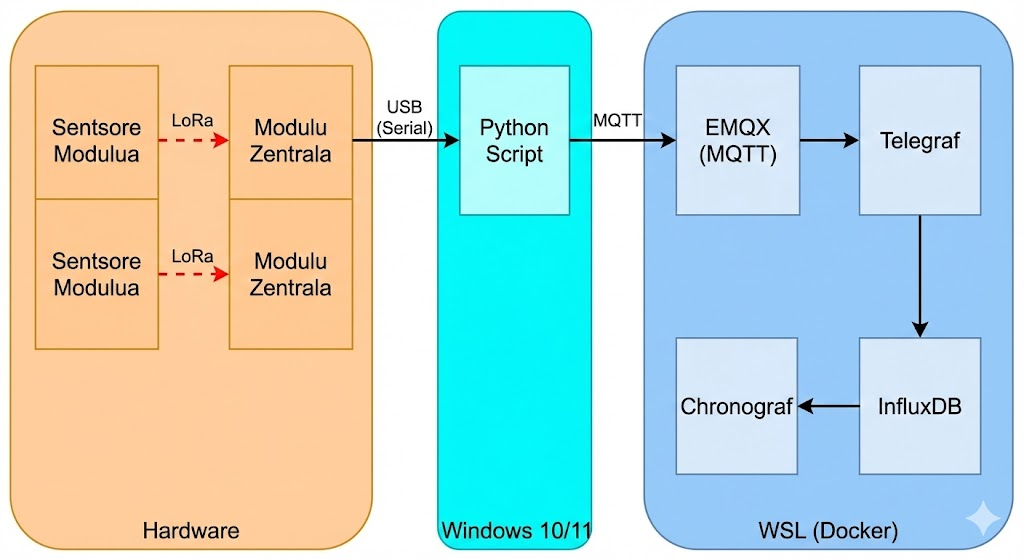
\includegraphics[width=0.9\textwidth]{Irudiak/IoT_Arkitektura_Finala.png}
    \caption{Inplementatutako \ac{IoT} arkitektura hibridoa}
    \label{fig:iot_final}
\end{figure}

\subsubsection{Edukiontzien Kudeaketa: Docker Compose}

Hasierako probetan edukiontzi bakoitza banan-banan exekutatzea (\texttt{docker run}) planteatu bazen ere, azkenean \texttt{docker-compose} tresna erabiltzea erabaki da. Tresna honek aukera ematen du aplikazio multi-edukiontzi bat definitzeko eta exekutatzeko \cite{turnbull2014docker}.\\

Gure kasuan, zerbitzu guztiak (EMQX, InfluxDB, Telegraf eta Chronograf) fitxategi bakar batean definitzen dira (\texttt{docker-compose.yml}). Fitxategi hau YAML formatuan idatzita dago eta bertan hiru atal nagusi zehazten dira:\\
\begin{enumerate}
    \item \textbf{Zerbitzuak:} Exekutatuko diren edukiontziak (InfluxDB, Telegraf, etab.), bakoitza bere irudiarekin eta portuekin.
    \item \textbf{Bolumenak:} Datuen iraupena bermatzen duten biltegiratze-eremuak. Horri esker, nahiz eta ordenagailua itzali edo edukiontziak berrabiarazi, datu-baseko informazioa ez da galtzen.
    \item \textbf{Sareak:} Edukiontzien arteko komunikazioa ahalbidetzen duen barne-sarea.
\end{enumerate}

Inplementazioan zehar, Telegraf zerbitzuarekin sinkronizazio arazo bat atzeman zen. Ondoko erregistroan ikus daitekeen bezala, Telegraf edukiontzia etengabe berrabiarazten zen hasieran:\\

\begin{lstlisting}[style=terminal]
gontz@Gontzal:/mnt/c/Users/gontz/PycharmProjects/TFG$ docker ps
CONTAINER ID   IMAGE            COMMAND                  CREATED        STATUS                          PORTS                          NAMES
a3c8d6d01c25   telegraf:latest  "/entrypoint.sh tele…"   14 hours ago   Restarting (1) Less than a second ago   8092/udp, 8125/udp, 8094/tcp   telegraf
\end{lstlisting}

Arazo hau lasterketa-baldintza (\textit{race condition}) baten ondorioa da: Docker-ek zerbitzu guztiak aldi berean abiarazten ditu, baina EMQX broker-ak denbora gehiago behar du guztiz operatibo egoteko Telegraf baino. Ondorioz, Telegraf konektatzen saiatzen denean, EMQX oraindik ez dago prest, eta errore ematen du. Arazo hau konpontzeko, \texttt{restart: always} politika ezarri zen konfigurazioan. Horrela, Telegraf-ek huts egiten badu, automatikoki berriro saiatzen da konexioa ezarri arte, sistemaren erresilientzia bermatuz.\\

\subsubsection{Telegraf-en Konfigurazioa}

Datuen bilketa eta bideratzea kudeatzeko, Telegraf agentea funtsezkoa da gure sisteman. Bere portaera \texttt{telegraf.conf} fitxategiaren bidez definitzen da. Fitxategi honek zehazten du nola jaso datuak (\textit{inputs}) eta nora bidali (\textit{outputs}).\\

Gure kasuan, \ac{MQTT} bidez jasotzen ditugu datuak JSON formatuan eta InfluxDB datu-basera bidaltzen ditugu. Konfigurazioaren zati garrantzitsuena honako hau da:\\

\begin{lstlisting}[style=terminal]
[agent]
  interval = "5s"
  round_interval = true
  metric_batch_size = 1000
  metric_buffer_limit = 10000
  collection_jitter = "0s"
  flush_interval = "5s"
  flush_jitter = "0s"

[[outputs.influxdb]]
  urls = ["http://influxdb:8086"]
  database = "sentsore_db"

[[inputs.mqtt_consumer]]
  servers = ["tcp://emqx:1883"]
  topics = ["sentsoreak/data"]
  data_format = "json"
\end{lstlisting}

Konfigurazio honetan ikus daitekeenez, agenteak 5 segundoro prozesatzen ditu datuak (\texttt{interval = ''5s''}). Sarrerako datuak \texttt{emqx} zerbitzarian entzuten dira \texttt{sentsoreak/data} gaian, eta irteera zuzenean \texttt{influxdb} zerbitzura bideratzen da, \texttt{sentsore\_db} datu-basera.\\

\subsubsection{Ibilbidea eta Ingurune Birtualak }

Arduino modulu zentraletik datuak jaso eta \ac{MQTT} broker-era bidaltzeko, Python script bat garatu da (\texttt{arduinopython.py}). Script honek bitartekari lana egiten du: datu gordinak formatu irakurgarri batera bihurtzen ditu. Zehazki, serieko portutik jasotako karaktere-kateak banatu eta JSON objektu egituratu batean bihurtzen ditu (timestamp, tenperatura, hezetasuna, etab.), Telegraf-ek erraz prozesatu ahal izateko.\\

Garapen honetan, mendekotasunen kudeaketa egokia ezinbestekoa izan da. Hasieran, sistema eragilearen Python instalazio orokorra erabiltzen saiatzean, liburutegien bertsio-gatazkak eta falta diren moduluen erroreak agertu ziren:\\

\begin{lstlisting}[style=terminal]
(base) PS C:\Users\gontz\PycharmProjects\TFG> python arduinopython.py
Traceback (most recent call last):
  File "C:\Users\gontz\PycharmProjects\TFG\arduinopython.py", line 1, in <module>
    import serial
ModuleNotFoundError: No module named 'serial'
\end{lstlisting}

Arazo hau konpontzeko eta garapen-ingurune garbia mantentzeko, \textbf{Conda} kudeatzailea erabili da ingurune birtual isolatu bat sortzeko (\texttt{TFG} izenekoa). Ingurune honek aukera ematen du proiektuaren mendekotasunak (\texttt{pyserial} eta \texttt{paho-mqtt}) bertsio zehatzetan instalatzeko, sistema eragileko beste proiektu batzuekin interferentziarik sortu gabe \cite{anaconda_conda}.\\

Bereziki garrantzitsua izan da \texttt{paho-mqtt} liburutegiaren 2.0 bertsiora egokitzea, \textit{Callback API} berria eskatzen baitu konexioak behar bezala kudeatzeko.\\

Laburbilduz, datuen fluxua honako hau da:\\
\begin{enumerate}
    \item Arduino MKR WAN 1310 plakak sentsoreen datuak jasotzen ditu \ac{LoRa} bidez.
    \item Windows-en exekutatzen den Python script-ak (\texttt{Conda} ingurunean) datuak irakurtzen ditu USB bidez eta JSON formatura bihurtzen ditu.
    \item Datuak \ac{MQTT} bidez bidaltzen dira \ac{WSL}-n exekutatzen ari den EMQX broker-era.
    \item Telegraf-ek mezuak harpatu eta InfluxDB datu-basean idazten ditu.
\end{enumerate}

\subsubsection{Datuen bistaratzea eta Konexio-katea}

Arkitekturaren erronka interesgarri bat Chronograf (bisualizazio tresna) eta InfluxDB (datu-basea) arteko konexioa ezartzea izan da. Hemen Docker-en barne-sarearen eta ostalariaren arteko bereizketa ulertzea ezinbestekoa izan da.\\

Erabiltzaileak Chronograf-era sartzeko nabigatzailean \texttt{http://localhost:8888} helbidea erabiltzen dugun arren, Chronograf-ek ezin du ''localhost'' erabili InfluxDB aurkitzeko \cite{influxdata_chronograf}. Docker edukiontziaren barruan, ''localhost'' Chronograf bera da. Horregatik, konexio-katean honako hau erabili behar izan da:\\

\begin{lstlisting}[style=terminal]
http://influxdb:8086
\end{lstlisting}

Hemen, ''influxdb'' ez da web domeinu bat, baizik eta \texttt{docker-compose.yml} fitxategian definitutako zerbitzuaren izena. Docker-ek izen hori automatikoki ebazten du barneko IP helbidera, bi edukiontzien arteko komunikazio zuzena ahalbidetuz.\\

Ondoko irudian ikus daiteke InfluxDB eta Chronografen arteko integrazioa, datuak denbora errealean bistaratzen diren panela erakutsiz:\\

\begin{figure}[H]
    \centering
    \IfFileExists{Irudiak/influx_dashboard.png}
    {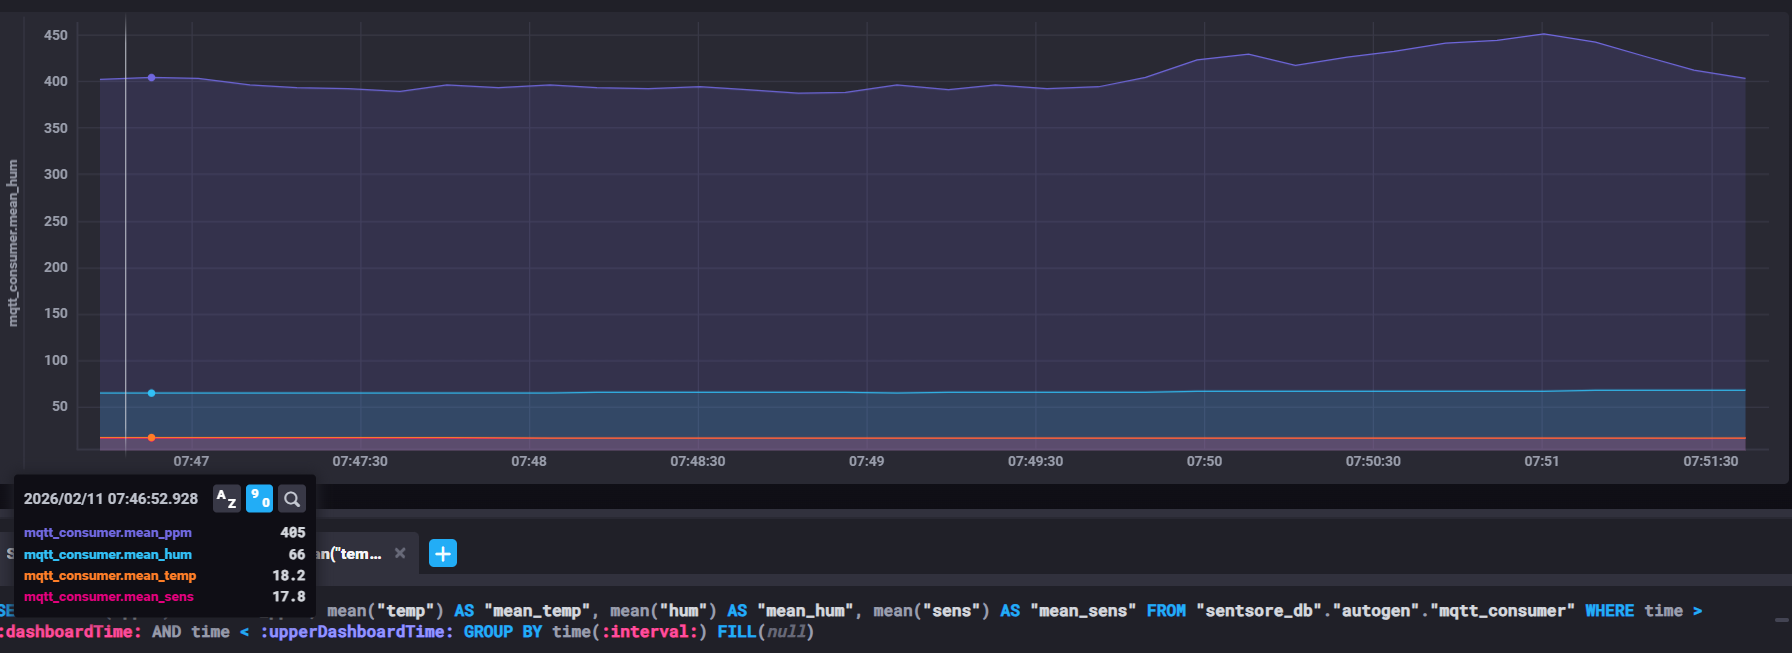
\includegraphics[width=0.9\textwidth]{Irudiak/influx_dashboard.png}}
    {\fbox{Irudia falta da: influx\_dashboard.png}}
    \caption{Chronograf panela datuak denbora errealean bistaratzen}
    \label{fig:influx_dashboard}
\end{figure}

\subsubsection{Zerbitzuen Kudeaketa}

Sistemaren integritatea mantentzeko, ezinbestekoa da edukiontziak modu ordenatuan kudeatzea. InfluxDB bezalako datu-base batek fitxategiak idazten dituen bitartean ordenagailua bat-batean itzaltzeak datu-galerak eragin ditzake. Hori ekiditeko, honako komando-protokoloa ezarri da \ac{WSL} terminalean:\\

\begin{itemize}
    \item \textbf{Zerbitzuak abiaraztea:} \texttt{docker-compose up -d} komandoak zerbitzu guztiak atzeko planoan (\textit{detached mode}) altxatzen ditu.
    \item \textbf{Egoera egiaztatzea:} \texttt{docker-compose ps} komandoak edukiontziak ''Up'' egoeran daudela baieztatzeko balio du.
    \item \textbf{Gelditze segurua:} Lan-saioa amaitzean, \texttt{docker-compose stop} komandoa erabiltzen da. Honek ''SIGTERM'' seinalea bidaltzen die edukiontziei, prozesuak (eta fitxategi-idazketak) modu ordenatuan itxi daitezen ordenagailua itzali aurretik.
\end{itemize}

\vspace{.3cm}

\section{Emaitza Esperimentalak}

Atal honetan garatutako sistemaren balioztatze esperimentala aurkezten da. Sistemaren egonkortasuna, erantzun-denbora eta irismena egiaztatzeko bi proba nagusi diseinatu eta burutu dira.\\

\subsection{Epe luzeko monitorizazioa eta egonkortasuna}

Sistemaren sendotasuna egiaztatzeko, gau osoan zeharreko etengabeko monitorizazioa burutu da. Proba honen helburua bi faktore nagusi balioztatzea izan da: batetik, datuen bilketan etenik ez dagoela bermatzea, eta bestetik, sentsoreek ingurune egonkor batean aldaketa txikiak detektatzeko duten sentsibilitatea neurtzea.\\

Jarraian aurkezten den grafikoan tenperaturaren eta airearen kalitatearen eboluzio naturala ikus daiteke ingurune itxi batean, gaueko 00:30etik 02:00etara bitartean:\\

\begin{figure}[H]
    \centering
    \IfFileExists{Irudiak/gaua.png}
    {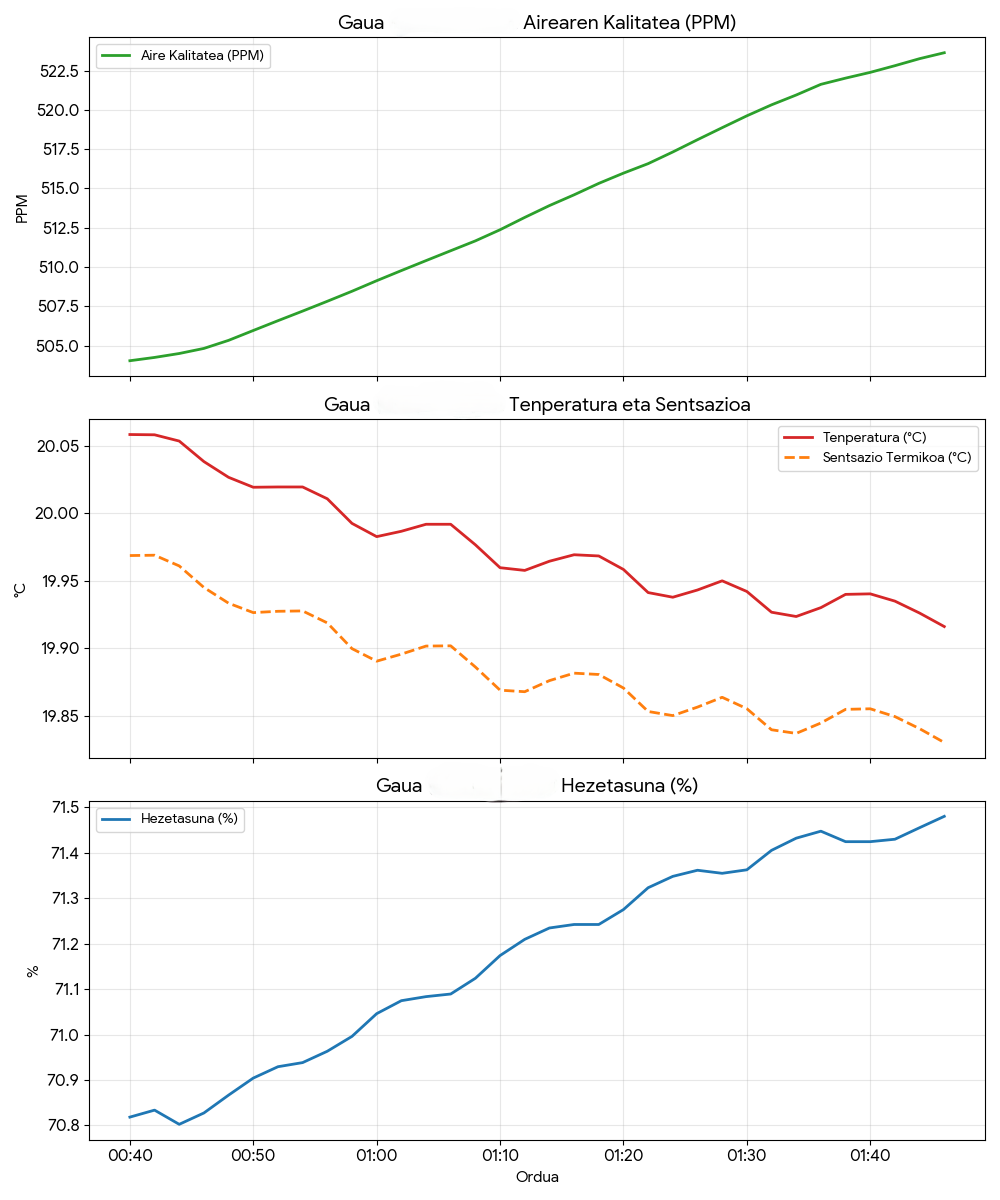
\includegraphics[width=0.85\textwidth]{Irudiak/gaua.png}}
    {} 
    \caption{Gaueko monitorizazioa: Tenperatura eta airearen kalitatea egonkor mantentzen dira}
    \label{fig:emaitzak_gaua}
\end{figure}

Emaitzek erakusten dutenez, sistemak sentsibilitate handia du ingurunearen aldaketa sotilak erregistratzeko. Tarte horretan (00:40 - 01:45), airearen kalitateak (PPM) goranzko joera arina erakutsi du, 505 PPMtik 523 PPMra igoz. Igoera txiki honek, gela itxi batean aireztapenik gabe metatzen den $CO_2$ kontzentrazioa islatzen du.\\

Aldi berean, tenperatura eta sentsazio termikoa 20,05ºC-tik 19,85ºC-ra jaitsi dira modu mailakatuan, gaueko tenperatura-galera naturala zehaztasunez jarraituz. Hezetasunari dagokionez, \%70,8tik \%71,5era igo da, tenperaturaren jaitsierarekin bat datorren portaera fisikoa erakutsiz (aire hotzak hezetasun erlatibo handiagoa izateko joera baitu). Datu hauek baieztatzen dute \ac{LoRa} bidezko transmisioa egonkorra dela eta pasarelak ez duela datu-galerarik eragiten, laginketa-frekuentzia konstante mantenduz.\\

\subsection{Ingurune-aldaketen detekzioa denbora errealean}

Sistemaren erantzun-denbora eta aldaketa bortitzen aurreko portaera aztertzeko, proba dinamiko bat egin da goizean. Gela itxi bateko leihoa ireki da minutu batzuez, kanpoko aire freskoa sar dadin, eta sentsoreen erreakzioa monitorizatu da.\\

\begin{figure}[H]
    \centering
    \IfFileExists{Irudiak/goiza.png}
    {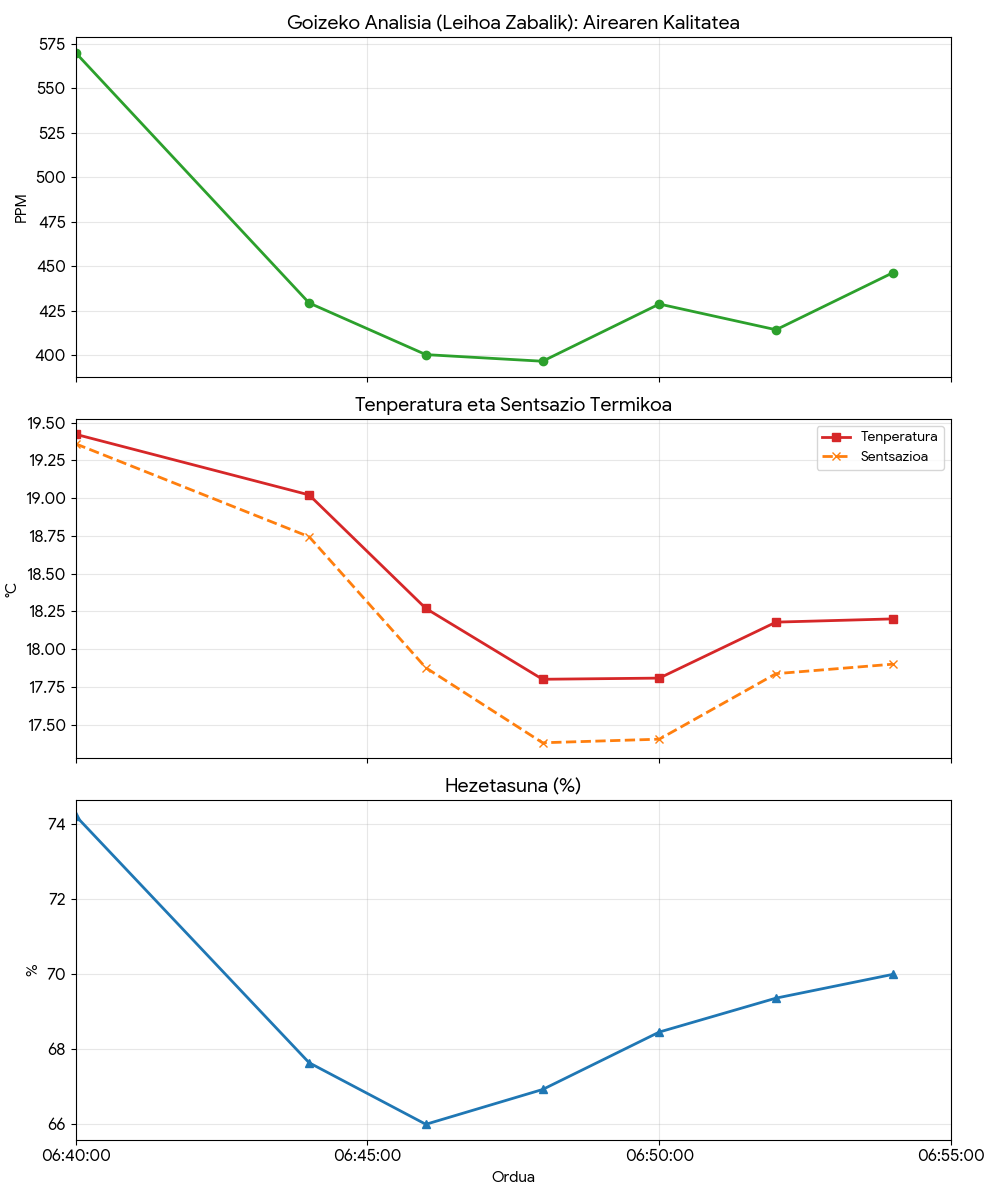
\includegraphics[width=0.85\textwidth]{Irudiak/goiza.png}}
    {} 
    \caption{Erantzun azkarra: Leihoa irekitzean tenperatura eta PPM mailak berehala jaisten dira}
    \label{fig:emaitzak_leihoa}
\end{figure}

Goiko grafikoan ikus daitekeenez, sistemak ia berehala detektatu ditu ingurune-aldaketak. Airearen kalitatea nabarmen hobetu da aireztapenaren ondorioz: balioak 575 PPM ingurutik (grafikoan ikusten den pikoaren aurretik) 400 PPMren azpira jaitsi dira minutu gutxian, kanpoko aire garbiaren mailara iritsiz.\\

Aldaketa termikoa ere oso nabaria izan da: tenperatura eta sentsazio termikoa 19,5ºC-tik 17,8ºC-ra jaitsi dira epe laburrean, sentsoreak korronte hotzak detektatzeko duen gaitasuna frogatuz. Hezetasuna, bestalde, \%74tik \%68ra jaitsi da, barruko aire kargatua kanpoko aire lehorragoarekin berritu dela adieraziz. Emaitza hauek frogatzen dute sistema gai dela denbora errealeko alerta-sistemetan erabiltzeko, aireztapen beharra edo tenperatura-galerak unean bertan identifikatzeko.\\

\subsection{LoRa irismenaren analisia}
\label{sec:irismena}

Azkenik, \ac{LoRa} teknologiaren gaitasun nagusia den irismena frogatzeko, eremu irekiko proba bat burutu da hiri-inguruneko kale batean. Proba honen helburua bikoitza izan da: batetik, bi moduluen arteko gehienezko distantzia neurtzea, eta, bestetik, seinalearen kalitatea (\textit{\ac{RSSI}} eta \textit{\ac{SNR}} parametroak) distantziarekin nola degradatzen den aztertzea.\\

\subsubsection{Proba-metodologia}

Probarako muntaia ondoko moduan prestatu da. Sentsore-modulua (igorlea) kale baten goiko muturrean kokatu da, ibilgailu baten gainean, lurretik gora altxatuta eta beheranzko inklinazio arin batekin. Kokapen altu honek garrantzi handia izan du emaitzetan: antenak ikuspegi-lerro (\textit{Line of Sight}, LOS) garbia izateak eta lehen Fresnel eremua lurretik eta oztopoetatik libre mantentzeak seinalearen hedapena nabarmen errazten baitute. Modulu zentrala (hargailua), aldiz, ordenagailura eta \ac{LCD} pantailara konektatuta eraman da eskuz, kalean behera pixkanaka urrunduz.\\

Irrati-parametroei dagokienez, proban zehar sistema errealean erabilitako konfigurazio bera mantendu da: 868 MHz-eko maiztasuna, 7ko zabaltze-faktorea (\textit{Spreading Factor}, SF), 125 kHz-eko banda-zabalera, 4/5 kodetze-tasa eta 17 dBm-eko transmisio-potentzia. Igorleak pakete bat bidaltzen du bi segundoro, kontagailu inkremental batekin; horrela, hargailuak distantzia bakoitzean galdutako paketeak zenbatu ditzake.\\

Neurketa-puntu bakoitzean, jasotako azken paketearen \ac{RSSI} (dBm-tan) eta \ac{SNR} (dB-tan) balioak \ac{LCD} pantailan erregistratu dira, baita kokapenaren GPS koordenatuak ere. Jasotako pakete bakoitzak hiru datu ditu serieko monitorean: pakete-kontagailua, \ac{RSSI} eta \ac{SNR}. \ref{fig:irismen_mapa}.irudian ibilbide osoa ikus daiteke, igorlearen kokapen finkotik (1.\ puntua) konexioa galdu den puntura arte (8.\ puntua).\\

\begin{figure}[H]
    \centering
    \IfFileExists{Irudiak/irismen_mapa.png}
    {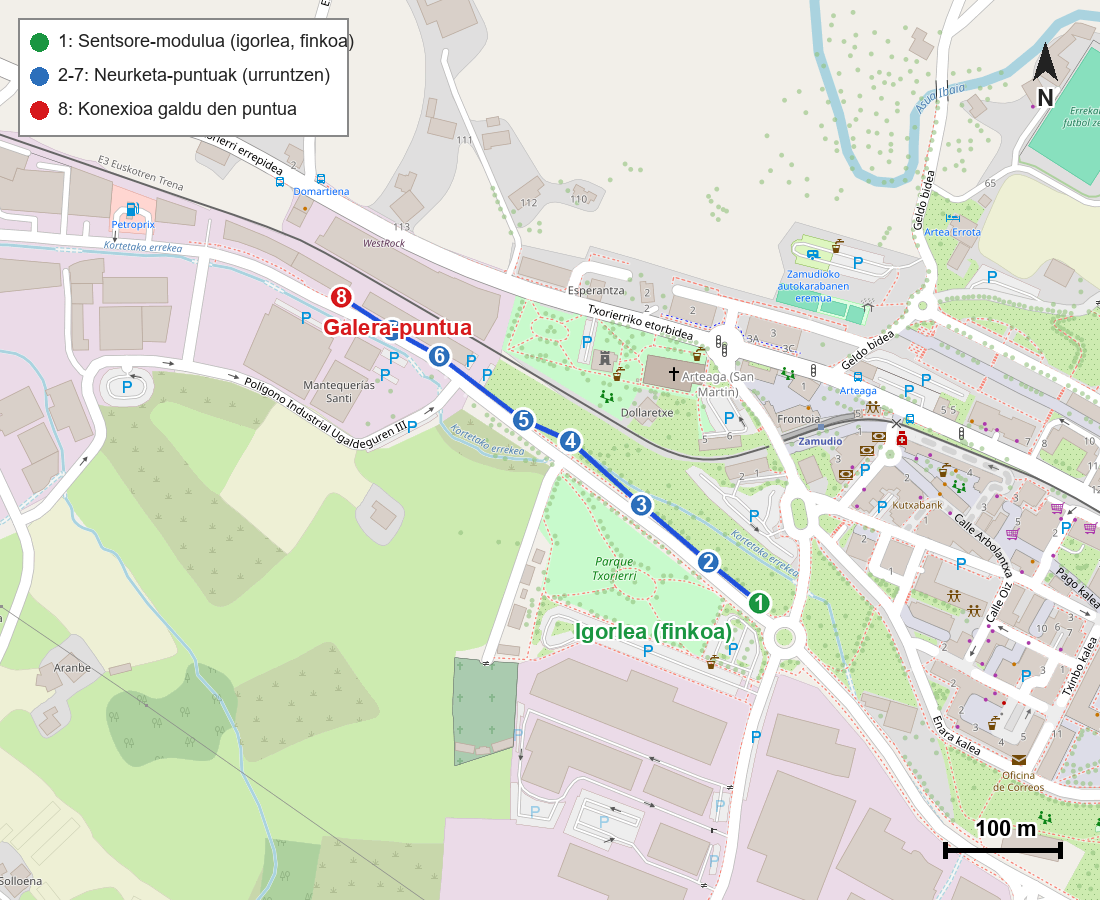
\includegraphics[width=0.92\textwidth]{Irudiak/irismen_mapa.png}}
    {\fbox{Irudia falta da: irismen\_mapa.png}}
    \caption{Irismen-probaren ibilbidea: igorlea (1.\ puntua, finkoa) eta neurketa-puntuak konexioa galdu arte (8.\ puntua, gorriz)}
    \label{fig:irismen_mapa}
\end{figure}

\ref{taula:irismen}.taulan puntu bakoitzaren arteko tarte-distantzia eta hasierako puntutik metatutako distantzia (lerro zuzenean) ageri dira. Ikus daitekeenez, konexioa galdu den unean bi moduluak \textbf{450 metrora} zeuden gutxi gorabehera, lerro zuzenean neurtuta; kalearen bihurguneak direla eta, oinez egindako distantzia handixeagoa izan da.\\

\begin{table}[H]
\centering
\begin{tabular}{c c c}
\hline
\textbf{Puntua} & \textbf{Tarte-distantzia (m)} & \textbf{Metatutako distantzia (m)} \\
\hline
1 (igorlea) & --- & 0 \\
2 & 56 & 56 \\
3 & 76 & 133 \\
4 & 83 & 216 \\
5 & 44 & 259 \\
6 & 92 & 351 \\
7 & 46 & 397 \\
8 (galera) & 53 & 450 \\
\hline
\end{tabular}
\caption{Neurketa-puntuen arteko distantziak (lerro zuzenean, GPS koordenatuetatik kalkulatuta)}
\label{taula:irismen}
\end{table}

\subsubsection{Seinalearen bilakaera: RSSI eta SNR}

\ref{fig:irismen_rssi}.irudian proban zehar jasotako \ac{RSSI} eta \ac{SNR} balioen bilakaera ageri da, serieko monitorean erregistratutako datuetatik abiatuta. Grafikoan probaren bost fase nabarmentzen dira:\\

\begin{itemize}
    \item \textbf{Seinale ona (hurbil):} hasieran, hargailua igorletik gertu zegoela, \ac{RSSI}a -90 eta -100 dBm bitartean mantendu da, eta \ac{SNR}a +7 eta +10 dB bitartean. Marjin zabala, konexioa guztiz egonkorra izanik.
    \item \textbf{Degradazioa:} urruntzen joan ahala, \ac{RSSI}a -120 dBm-ren azpira jaitsi da pixkanaka, eta \ac{SNR}a balio negatiboetara igaro da.
    \item \textbf{Sentsibilitate-muga:} \ac{RSSI}a -126/-127 dBm inguruan ``ainguratu'' da, hargailuaren sentsibilitate-muga praktikoa adieraziz. Fase honetan, kontagailu ilegigarriko paketeak agertu dira (irudian markatuak), hau da, errorez jasotako paketeak, seinalea zarataren mailan dagoenaren seinale argia.
    \item \textbf{Konexioa ia galduta:} fase honetan pakete oso gutxi iritsi dira (kontagailuan jauzi handiak), bihurgune baten ondoren igorlea ikuspegitik galdu denean.
    \item \textbf{Berreskurapena:} itzuleran, ikuspegi-lerroa berreskuratzean, \ac{RSSI}a berriro igo da (-110/-118 dBm) eta \ac{SNR}a balio positiboetara itzuli da.
\end{itemize}

\begin{figure}[H]
    \centering
    \IfFileExists{Irudiak/irismen_rssi_snr.png}
    {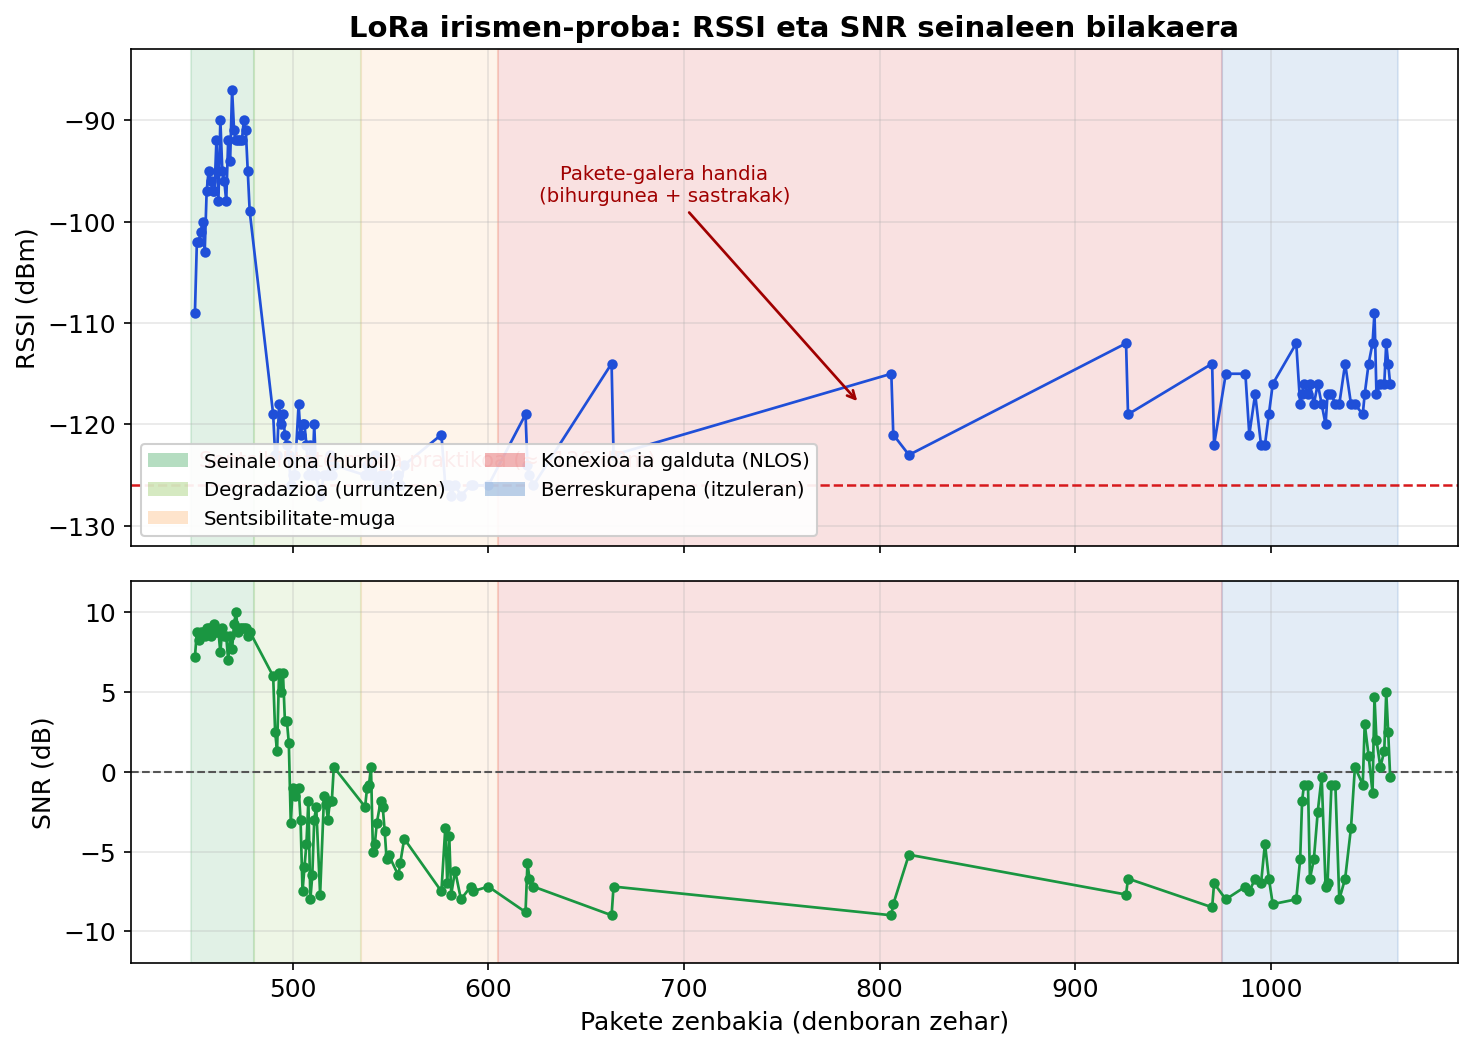
\includegraphics[width=\textwidth]{Irudiak/irismen_rssi_snr.png}}
    {\fbox{Irudia falta da: irismen\_rssi\_snr.png}}
    \caption{\ac{RSSI} eta \ac{SNR} seinaleen bilakaera proban zehar, faseka koloreztatuta}
    \label{fig:irismen_rssi}
\end{figure}

\ac{LCD} pantailan zuzenean ikus zitekeen degradazio hau. \ref{fig:irismen_lcd}.irudian bi une alderatzen dira: ezkerrean, igorletik gertu (\ac{RSSI} = -92 dBm, \ac{SNR} = +9,0 dB), eta eskuinean, ia muturrean (\ac{RSSI} = -123 dBm, \ac{SNR} = -5,2 dB). \\

\begin{figure}[H]
    \centering
    \IfFileExists{Irudiak/irismen_lcd_hurbil.jpg}
    {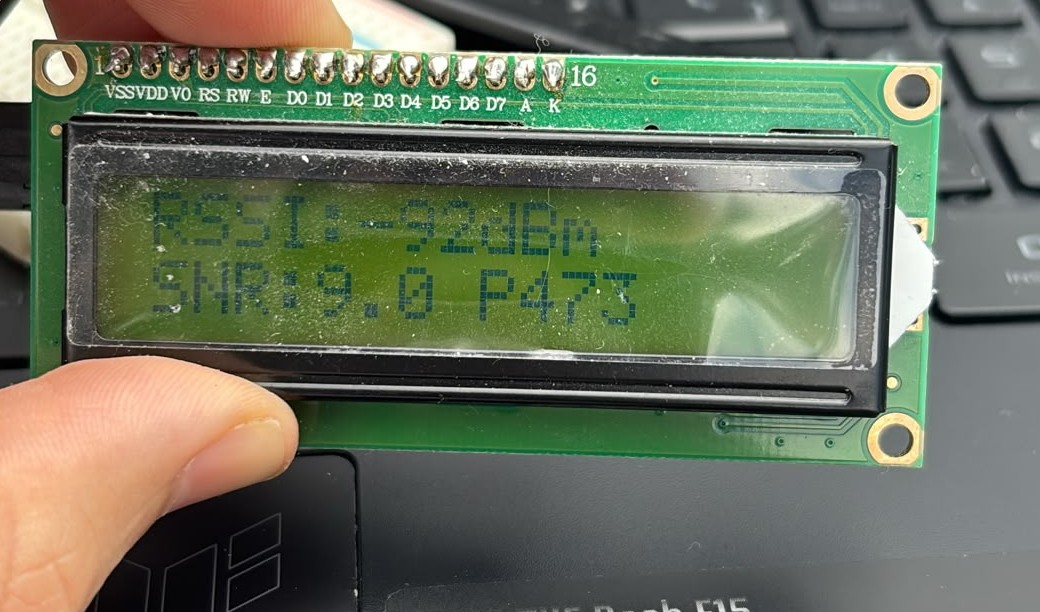
\includegraphics[width=0.48\textwidth]{Irudiak/irismen_lcd_hurbil.jpg}}
    {\fbox{\parbox[c][3cm]{0.48\textwidth}{\centering Irudia falta da}}}
    \hfill
    \IfFileExists{Irudiak/irismen_lcd_urrun.jpg}
    {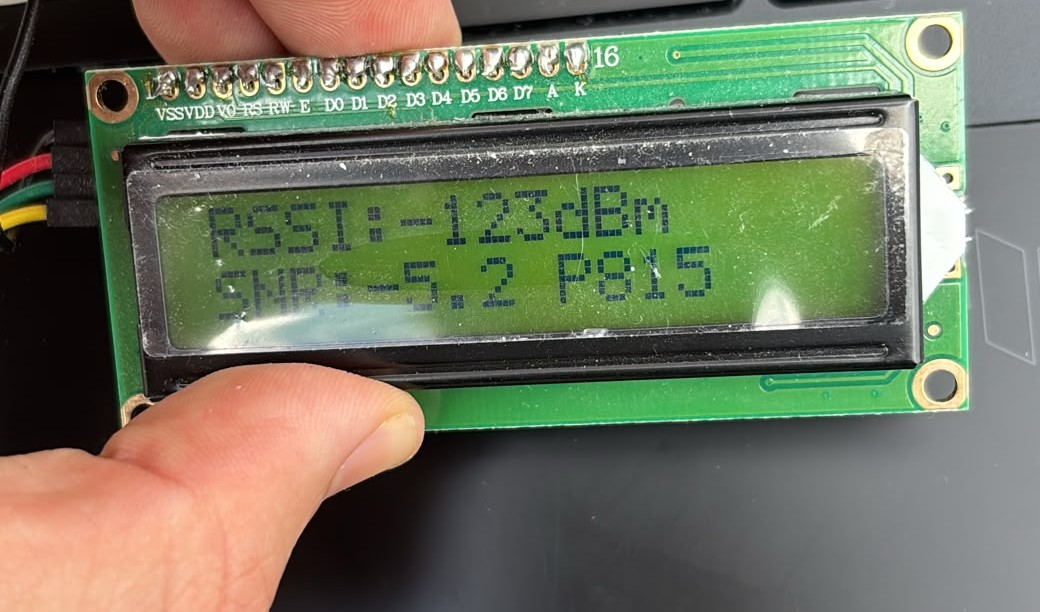
\includegraphics[width=0.48\textwidth]{Irudiak/irismen_lcd_urrun.jpg}}
    {\fbox{\parbox[c][3cm]{0.48\textwidth}{\centering Irudia falta da}}}
    \caption{Modulu zentraleko \ac{LCD} pantaila bi distantziatan: gertu (ezkerrean, RSSI -92 dBm) eta urrun (eskuinean, RSSI -123 dBm)}
    \label{fig:irismen_lcd}
\end{figure}

\subsubsection{Konexioaren galera eta berreskurapena}

Probaren emaitzarik interesgarriena seinalea galtzeko moduan datza. Sentsibilitate-mugara iristean, konexioa ezegonkor bihurtu da: hargailua geldituz gero, seinalea berreskuratu egiten zen, baina mugituz gero, berriz galtzen zen tarteka. Portaera hau muga-mugako esteka baten ezaugarri tipikoa da; \ac{RSSI}a -127 dBm-tan dagoenean, marjina hain da txikia, ezen kokapen-aldaketa txikiek (\textit{multipath} edo seinale-desbanezimenduak) nahikoa baitira muga gainditzeko norabide batean edo bestean.\\

Konexioaren erabateko galera, ordea, ez da distantziak soilik eraginda gertatu, baizik eta ikuspegi-lerroa galtzeagatik. 8.\ puntuaren ondoren, kaleak ezkerrera egiten zuen bihurgune bat zuen, eta, bertan, sastrakak zeuden bidearen ertzean. Igorlea ikuspegitik desagertu eta ikuspegi-lerrorik gabeko egoerara (\textit{Non-Line-of-Sight}, NLOS) igarotzean, seinalea erabat galdu da. Landaredia bereziki erasokorra da maiztasun hauetan, eta horregatik ez da konexioa berreskuratu igorlea berriro ikusgai egon arte. Hain zuzen ere, itzuleran, ibilgailua berriro begien aurrean izan dugunean, konexioa berehala berreskuratu da.\\

Emaitza honek probaren ondoriorik garrantzitsuena berresten du: \ac{LoRa} estekaren faktore kritikoa ez da distantzia hutsa, baizik eta \textbf{ikuspegi-lerroa eta antenaren altuera}. Ikuspegi-lerro garbiarekin 450 metroko irismena lortu da hiri-ingurunean; aldiz, oztopo hurbil batek (bihurgunea eta sastrakak) nahikoa izan da esteka erortzeko, distantzia txikiagoa izan arren ere.\\

Laburbilduz, proba honek erakutsi du diseinatutako sistemak \textbf{400-450 metro inguruko irismen egonkorra} eskaintzen duela ikuspegi-lerroko hiri-ingurunean, sentsore-sare baten aplikazio errealetarako (adibidez, eraikin bateko gela edo solairu desberdinen monitorizazioa) guztiz nahikoa den tartea.\\

\subsection{RadioLib liburutegira migrazioa eta zabaltze-faktorearen azterketa}
\label{sec:radiolib}

Sistemaren oinarrizko helburuak bete ondoren, bikaintasunera bideratutako hedapen gisa eta zuzendaritzak iradokita, sistemaren irrati-geruza \textbf{RadioLib} \cite{radiolib} liburutegira migratu da. Migrazio honek aukera eman du zabaltze-faktoreak (\textit{Spreading Factor}, SF) irismenean duen eragina modu kontrolatuan aztertzeko.\\

\subsubsection{Zergatik RadioLib}

Orain arte, \ac{LoRa} bidezko komunikazioa Sandeep Mistry-ren \texttt{LoRa.h} liburutegiarekin \cite{arduinolora} inplementatu da. Liburutegi horrek SX127x familiako txipekin bakarrik egiten du lan, eta parametroen kontrol mugatua eskaintzen du. RadioLib, aldiz, irrati-txip askotarako liburutegi unibertsal bat da (SX127x, SX126x, eta abar), eta hainbat abantaila eskaintzen ditu: irrati-hardware desberdinen arteko \textbf{eramangarritasuna}, irrati-parametroen \textbf{kontrol zehatza}, etenaldietan oinarritutako harrera (\textit{interrupt-driven}) eta mantentze-lan aktiboa. Ezaugarri horiek bereziki erabilgarriak dira etorkizuneko hobekuntzetarako (adibidez, errepikagailu bidezko sareak edo txip eraginkorragoetara migratzea).\\

\subsubsection{MKR WAN 1310-eko inplementazioa}

Migrazioaren erronka nagusia plakaren arkitekturan datza. Arduino MKR WAN 1310-ek SX1276 txipa Murata modulu baten barruan integratuta dauka, eta, txip horrekin zuzenean komunikatzeko, bi baldintza bete behar dira: irratiak \textbf{SPI1} busa erabiltzen du (200 kHz-tan; 2 MHz-eko abiadura lehenetsiak ez du funtzionatzen), eta modulua ``passthrough'' moduan jarri behar da hasieratzean, reset-sekuentzia berezi baten bidez. RadioLib-en konfigurazioa honako hau da:\\

\begin{lstlisting}[style=terminal]
// SX1276 interno del MKR WAN 1310 por SPI1 (CS=28, DIO0=31)
SX1276 radio = new Module(LORA_IRQ_DUMB, LORA_IRQ, RADIOLIB_NC,
               RADIOLIB_NC, SPI1, SPISettings(200000, MSBFIRST, SPI_MODE0));

// ...en setup(), antes de radio.begin():
//   reset del modulo Murata (LORA_IRQ_DUMB, LORA_BOOT0, LORA_RESET)
//   SPI1.begin();
int estado = radio.begin(868.0, 125.0, SF, 5, 0x12, 17, 8); // freq,BW,SF,CR,sync,TX,preamb
\end{lstlisting}

\subsubsection{Zabaltze-faktorearen eragina: SF7 vs SF12}

\ac{LoRa}-ren \ac{CSS} modulazioan, zabaltze-faktoreak datu-tasaren eta sentsibilitatearen arteko konpromisoa ezartzen du. SF altuago batek \textit{chirp} luzeagoak erabiltzen ditu: datu-tasa jaisten du, baina hartzailearen sentsibilitatea (eta, beraz, irismena) handitzen du. \ref{taula:sf}.taulan bi muturreko konfigurazioak alderatzen dira, 125 kHz-eko banda-zabalerarako.\\

\begin{table}[H]
\centering
\begin{tabular}{l c c}
\hline
\textbf{Parametroa} & \textbf{SF7} & \textbf{SF12} \\
\hline
Datu-tasa (gutxi gorabehera) & $\sim$5470 bps & $\sim$290 bps \\
Aireko denbora (pakete txikia) & $\sim$50 ms & $\sim$1000 ms \\
Sentsibilitatea (BW 125 kHz) & $\sim$-123 dBm & $\sim$-137 dBm \\
Neurtutako irismena (LOS) & 450 m & $\sim$775 m (eta gehiago) \\
\hline
\end{tabular}
\caption{SF7 eta SF12 konfigurazioen arteko alderaketa (125 kHz)}
\label{taula:sf}
\end{table}

Puntu fisiko garrantzitsu bat azpimarratu behar da: distantzia jakin batean jasotako \ac{RSSI} balioa ez dago SF-aren mende, transmisio-potentzia eta hedapen-bidea berberak baitira; aldatzen den bakarra hartzaileak deskodetu dezakeen gutxieneko maila da. SF7-k $\sim$-123 dBm-ra arte deskodetzen du; SF12-k, berriz, $\sim$-137 dBm-ra arte \cite{sx1276datasheet}. Esteka-aurrekontuan irabazitako $\sim$14 dB horiek irismena nabarmen luzatzen dute. Hori dela eta, aurreko atalean SF7-rekin neurtutako \ac{RSSI}-distantzia kurba berbera baliagarria da SF12-rako ere: SF7-k esteka galdu zuen punturaino ($\sim$-126 dBm), SF12-k erraz mantenduko luke konexioa, eta horrek frogatzen du SF12 konfigurazioak aplikazio bera tarte handiagoetara hedatzeko aukera ematen duela, datu-tasa baxuagoaren truke.\\

\subsubsection{Landa-probaren emaitzak (SF12)}

SF12 konfigurazioa RadioLib-ekin inplementatu ondoren, aurreko eguneko proba bera errepikatu da: igorlea (sentsore-modulua) kokapen berean utzi da eta ibilbide bera egin da. Emaitzak espero baino hobeak izan dira. SF7-rekin esteka galdu zen punturaino ($\sim$450 m) iritsita, SF12-k konexioa arazorik gabe mantendu du, eta hargailua askoz urrunago eraman ahal izan da: \textbf{$\sim$775 metrora arte} GPS bidez neurtuta, eta puntu horretatik harago ere paketeak jasotzen jarraitu du. \ref{fig:sf12_mapa}.irudian bi proben (SF7 eta SF12) alderaketa geografikoa ikus daiteke.\\

\begin{figure}[H]
    \centering
    \IfFileExists{Irudiak/irismen_sf12_mapa.png}
    {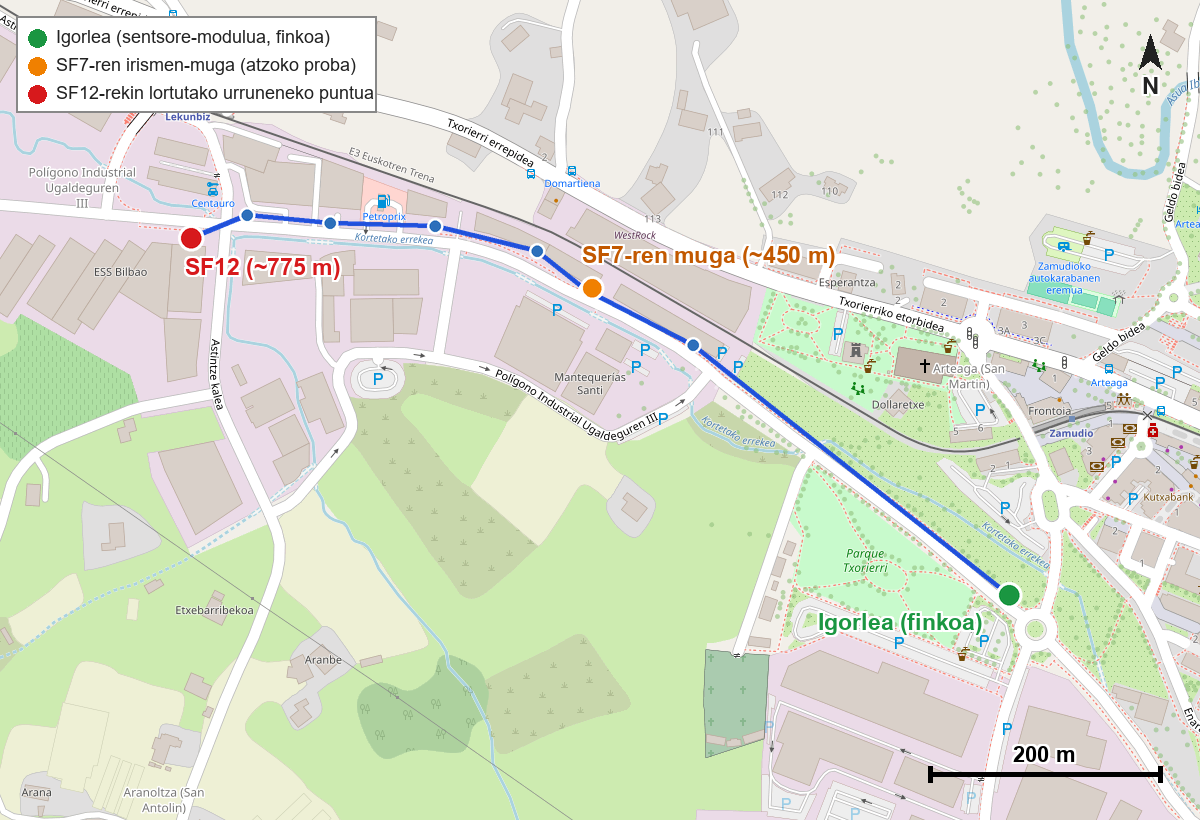
\includegraphics[width=0.95\textwidth]{Irudiak/irismen_sf12_mapa.png}}
    {\fbox{Irudia falta da: irismen\_sf12\_mapa.png}}
    \caption{SF7 eta SF12 proben alderaketa geografikoa: SF12-k SF7-ren irismen-muga ($\sim$450 m) gainditu eta $\sim$775 metrora arte iritsi da}
    \label{fig:sf12_mapa}
\end{figure}

\ref{fig:sf12_rssi}.irudian SF12-rekin jasotako 145 paketeren \ac{RSSI} eta \ac{SNR} balioen bilakaera osoa ageri da. Datu esanguratsuena \ac{RSSI}-aren gutxieneko balioa da: \textbf{-140 dBm}-eraino jaitsi da, hau da, SX1276 txiparen SF12 sentsibilitate-muga nominala ($\sim$-137 dBm) baino baxuagoa, eta, hala ere, paketeak zuzen deskodetzen jarraitu du. \ac{SNR}-ak, era berean, -20 dB-eraino egin du behera. Hori da, hain zuzen ere, SF altuen abantaila nagusia: zaratapeko komunikazioa (\textit{below noise floor}), SF7-rekin ezinezkoa zena.\\

\begin{figure}[H]
    \centering
    \IfFileExists{Irudiak/irismen_sf12_rssi.png}
    {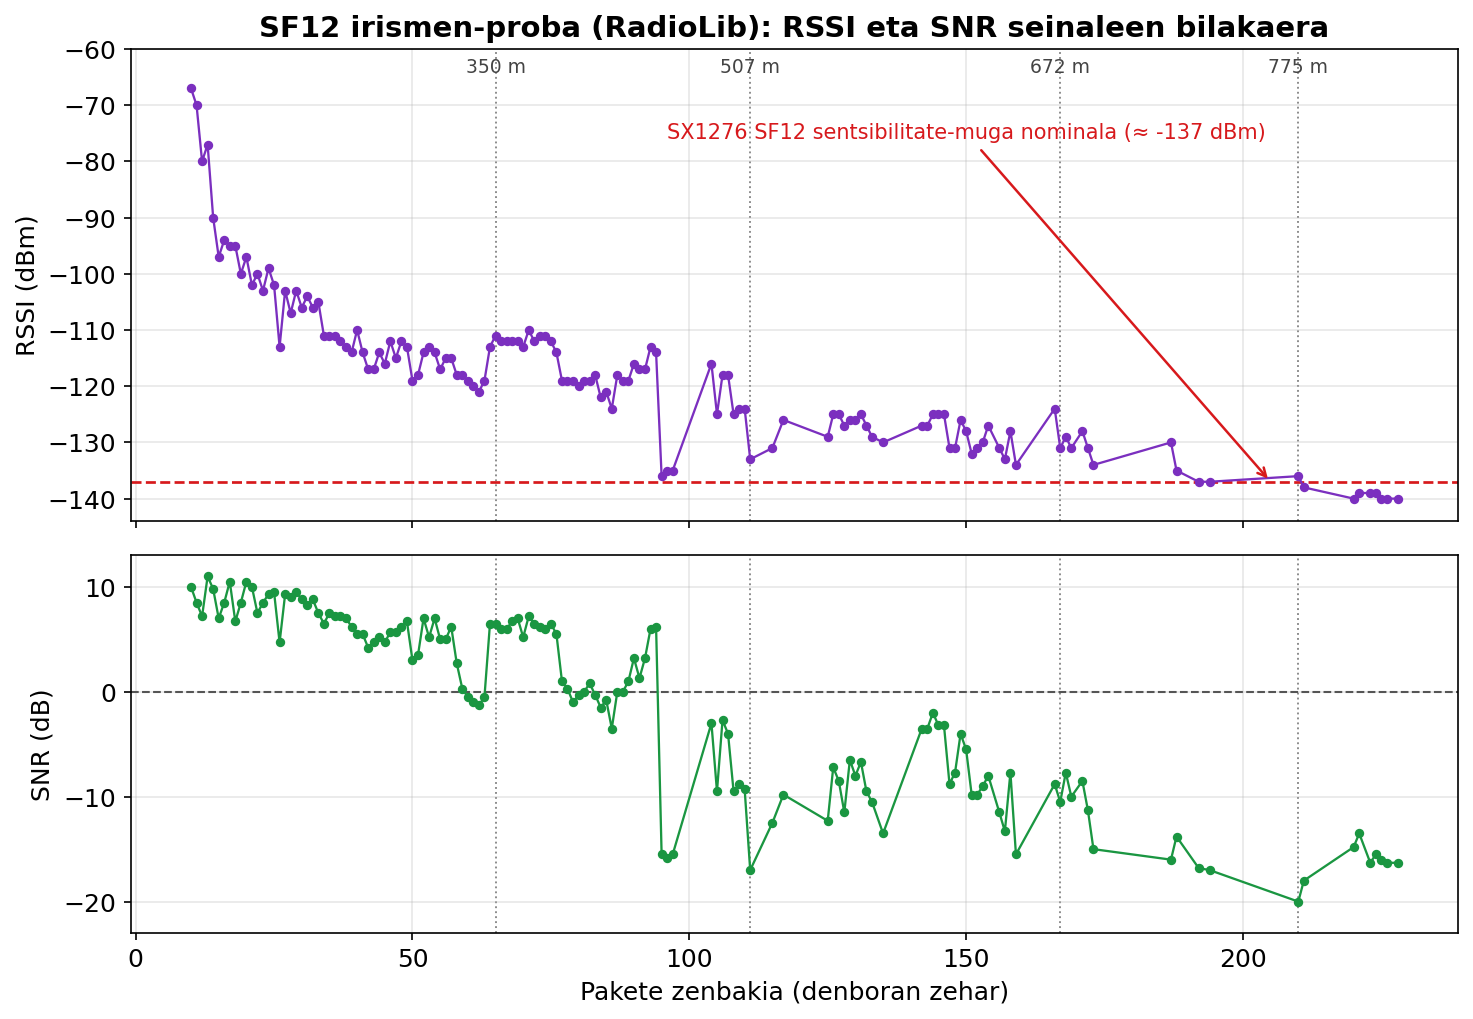
\includegraphics[width=\textwidth]{Irudiak/irismen_sf12_rssi.png}}
    {\fbox{Irudia falta da: irismen\_sf12\_rssi.png}}
    \caption{SF12 (RadioLib): \ac{RSSI} eta \ac{SNR}-aren bilakaera proba osoan zehar (145 pakete), goian distantzia adierazgarriekin}
    \label{fig:sf12_rssi}
\end{figure}

\ref{taula:sf12}.taulan ibilbideko neurketa-puntu georreferentziatuak laburbiltzen dira:\\

\begin{table}[H]
\centering
\begin{tabular}{c c c c}
\hline
\textbf{Pakete} & \textbf{Distantzia (m)} & \textbf{RSSI (dBm)} & \textbf{SNR (dB)} \\
\hline
10  & $\sim$60 (hasiera) & -67 & +10,0 \\
65  & 350 & -111 & +6,5 \\
95  & 453 & -136 & -15,5 \\
111 & 507 & -133 & -17,0 \\
142 & 592 & -127 & -3,5 \\
167 & 672 & -131 & -10,5 \\
187 & 740 & -130 & -16,0 \\
210 & 775 & -136 & -20,0 \\
220--228 & $>$775 & -140 & $\sim$-16 \\
\hline
\end{tabular}
\caption{SF12 probako neurketa-puntu georreferentziatuak (igorlea atzoko hasiera-puntuan)}
\label{taula:sf12}
\end{table}

Emaitza hauetatik hainbat ondorio interesgarri atera daitezke. Lehenik, $\sim$450 m-ko puntuan (atzo SF7-k esteka galdu zuen tokia) ordenagailua lurrean jartzean seinalea -136 dBm-ra jaitsi zen, eta altxatzean hobetu egin zen; horrek antenaren altueraren garrantzia berresten du. Bigarrenik, \ac{RSSI}-aren bilakaera oso leuna eta jarraitua izan da distantziarekin, esteka egonkorraren seinale. Eta, hirugarrenik, azken puntuetan, igorlea ikuspegitik galtzen hasita, konexioa lortzea kostatzen bazen ere, probak argi utzi du distantzia are handiagoetan esteka posible izango zatekeela.\\

Laburbilduz, \texttt{LoRa.h}-tik RadioLib-era migratzeak eta SF7-tik SF12-ra pasatzeak \textbf{irismena ia bikoiztea} ekarri du ($\sim$450 m-tik $\sim$775 m-ra), antena sinpleekin eta hiri-ingurunean. Aldaketa horren kostua datu-tasaren jaitsiera da (SF12-k $\sim$290 bps soilik), baina sentsore-sare baten aplikaziorako (noizean behingo neurketa txikiak) guztiz onargarria da.



% --- ONDORIOAK ETA ETORKIZUNEKO LANAK (INTEGRATUA) ---
\section{Ondorioak eta Etorkizuneko Lanak}

Lan honen garapenak aukera eman du \ac{LoRa} teknologian oinarritutako sentsore-sare malgu eta funtzional bat diseinatu eta inplementatzeko, hasieran ezarritako helburu guztiak arrakastaz betez. Proiektua ez da soilik datuak biltzera mugatu; hardwarearen eta softwarearen arteko integrazio sakona eskatu du, sentsore fisikoetatik hasi eta hodeiko bistaratze-sistemetaraino doan ibilbide osoa estaliz.\\

Proiektuaren ekarpen nagusietako bat garatutako sistemaren \textbf{bideragarritasun ekonomikoa} da. Merkatuan dauden soluzio komertzial garestien aldean, hemen aurkeztutako sistemak (bi moduluak eta sentsoreak barne, ordenagailua kontuan hartu gabe) \textbf{100 euro inguruko kostua} du. Ikerketek frogatu dutenez, kostu baxuko hardwarean oinarritutako \ac{IoT} sistemek monitorizazio profesional eta eskuragarria ahalbidetzen dute, zehaztasun maila onargarria mantenduz ingurune askotarako \cite{kumar2019low}.\\

Alderdi teknikorik konplexuena eta ikerketa-ordu gehien eskatu dituena moduluen arteko komunikazioaren kudeaketa izan da. \ac{LoRa} moduluak distantzia luzeetara datuak bidaltzeko bikainak diren arren, \textbf{bi noranzkoko komunikazioa} lortzea erronka handia izan da. Garapen-fasean, sistemak sarritan saturatu egiten ziren talken ondorioz. Arazo hau konpontzeko, software bidezko sinkronizazio zorrotza inplementatu da tenporizadore espezifikoekin. Doikuntza honek frogatu du \ac{LoRa} sentsore-sare sendoak sortzeko gai dela, baldin eta denbora-kudeaketa egokia aplikatzen bada.\\

Software-arkitekturari dagokionez, ingurune hibridoa (\ac{WSL} eta Windows) eta Docker bidezko edukiontziak erabiltzea erabaki estrategiko egokia izan da. Horrek sistema modularra eta eskalagarria bihurtu du: zerbitzu bat eguneratu edo aldatu behar bada, ez du eraginik gainerako sisteman. Gainera, Python bidez garatutako pasarelak zubi-lan eraginkorra egin du hardwarearen eta zerbitzarien artean.\\

Lortutako emaitza esperimentalek sistemaren fidagarritasuna berresten dute. Gaueko probetan ikusi den bezala, sistemak gai dira ingurumen-joerak zehaztasunez erregistratzeko zarata elektronikoa iragaziz. Are garrantzitsuagoa dena, goizeko probetan, leihoa irekitzean gertatutako aldaketa bortitzak berehala detektatu dira, sistema hau denbora errealeko alerta-sistemetarako baliagarria dela frogatuz.\\

Bestalde, irismen-probak \ac{LoRa} teknologiaren gaitasun bereizgarria baieztatu du: ikuspegi-lerroan, sistemak \textbf{400-450 metroko estaldura egonkorra} lortu du hiri-ingurunean. Proba horrek, gainera, agerian utzi du esteka-kalitatearen faktore erabakigarria ez dela distantzia hutsa, baizik eta ikuspegi-lerroa eta antenaren altuera. Azkenik, bikaintasunari begira, irrati-geruza RadioLib liburutegira migratu da; horri esker, zabaltze-faktorea (SF) doitu daiteke irismena are gehiago handitzeko, datu-tasa baxuagoaren truke.\\

\subsection*{Etorkizuneko Lanak}

Garatutako sistemak oinarri sendoa eskaintzen du etorkizuneko hobekuntzak txertatzeko, bereziki lortutako komunikazio bidirekzionalari esker:\\

\begin{itemize}
    \item \textbf{Sarearen eskalagarritasuna eta Errepikagailuak:} Lortutako ''dualitateak'' (nodoek entzun eta hitz egiteko gaitasuna izateak) aukera ematen du sentsore-moduluak \textbf{errepikagailu} gisa erabiltzeko. Etorkizunean, sarea hedatu liteke jauzi anitzeko sistema bat sortuz: Modulu Zentrala $\rightarrow$ A Modulua $\rightarrow$ B Modulua. Horrela, adibidez, ikastetxe batean klasez klaseko estaldura lor liteke modulu zentral bakarra erabiliz, seinalea batetik bestera pasatuz.
    
    \item \textbf{Autosufizientzia Energetikoa:} Proiektu honetan bateria kargagarriak erabili dira sentsore-moduluak elikatzeko. Hasiera batean eguzki-plaken erabilera aztertu bazen ere, ideia baztertu egin zen aplikazioaren helburua barnealdeko espazioak (ikasgelak) monitorizatzea delako, non argi natural zuzena ez den nahikoa sistema elikatzeko. Hala ere, sistema hau kanpoaldean aplikatuko balitz, eguzki-energia integratzea litzateke hurrengo pauso logikoa.
    
    \item \textbf{Segurtasuna eta Kalibrazioa:} Gaur egun datuak irekian bidaltzen badira ere, enkriptatze-algoritmoak (AES-128) gehitzeak sarea ingurune publikoetan hedatzea ahalbidetuko luke \cite{daud2018securing}. Bestalde, MQ-135 sentsorea joerak neurtzeko egokia den arren, kalibrazio profesionalago batek balio absolutu zehatzak emango lituzke \cite{spinelle2015field}.
\end{itemize}
\newpage

% Basque babel-ek '~' aktibo bihurtzen du (ñ atajoa); bibliografiako egile-izenetako
% zuriune ez-hausgarriak (J.~Nickoloff) hausten ditu. Hemen '~' zuriune normal gisa uzten da.
\shorthandoff*{~}
\bibliographystyle{IEEEtran}
\bibliography{Bibliografia}

\newpage

\section*{Datasheet-ak}

\begin{enumerate}
    \item Sentsoreen datasheet-ak:
    \begin{itemize}
        \item \href{https://digizone.com.ve/wp-content/uploads/2022/02/MQ-135_Hanwei.pdf}{MQ-135}
        \item \href{https://www.mouser.com/datasheet/2/758/DHT11-Technical-Data-Sheet-Translated-Version-1143054.pdf}{DHT11} / \href{https://github.com/adafruit/DHT-sensor-library}{DHT sensor library by Adafruit}
    \end{itemize}
    \item \href{https://docs.arduino.cc/hardware/mkr-wan-1310}{Arduino MKR WAN 1310}
    \begin{itemize}
        \item \href{https://www.semtech.com/products/wireless-rf/lora-connect/sx1276}{Semtech SX1276 (LoRa transceiver-aren datasheet-a)}
    \end{itemize}

    \item \href{https://www.handsontec.com/dataspecs/module/I2C_1602_LCD.pdf}{I2C Serial Interface 1602 LCD Module}
    \begin{itemize}
        \item \href{https://docs.arduino.cc/learn/communication/wire}{Inter-Integrated Circuit (I2C) Protocol}
    \end{itemize}
    \item \href{https://www.electronicoscaldas.com/datasheet/LTE12-Series.pdf}{Active Buzzer}
    
    \item Software eta Liburutegiak:
        \begin{itemize}
            \item \href{https://github.com/jgromes/RadioLib}{RadioLib (jgromes) -- LoRa irrati-liburutegi unibertsala}
            \item \href{https://github.com/sandeepmistry/arduino-LoRa}{Arduino-LoRa (Sandeep Mistry)}
            \item \href{https://pypi.org/project/paho-mqtt/}{Paho-MQTT 2.0 (Python Client)}
            \item \href{https://pypi.org/project/pyserial/}{PySerial (Python Serial Port Extension)}
            \item \href{https://matplotlib.org/}{Matplotlib (Python Plotting Library)}
            \item \href{https://pandas.pydata.org/}{Pandas (Data Analysis \& Manipulation)}
            \item \href{https://docs.conda.io/en/latest/}{Conda Package Management System}
        \end{itemize}
\end{enumerate}

\end{document}